\section{Operationsverstaerker}

\subsection{Eigenschaften eines OpAmps}

\begin{minipage}{0.6\columnwidth}
	\begin{center}
		% LTeX: enabled=false
\resizebox{0.6\columnwidth}{!}{
    \begin{circuitikz}
        \tikzstyle{every node}=[font=\Huge]
        \draw [line width=1pt, short] (0,0) -- (7.75,4.5);
        \draw [line width=1pt, short] (0,0) -- (0,9);
        \draw (4.25,4.5) to[american voltage source] (2.75,3);
        \draw [line width=1pt, short] (7.75,4.5) -- (0,9);
        \node at (1,2.5) {\textbf{+}};
        \node at (1,6.5) {\textbf{-}};
        \draw (0.5,2.5) to[european resistor] (0.5,6.5);
        \draw (0.5,2.5) to[short, -o] (-1.75,2.5) ;
        \draw (0.5,6.5) to[short, -o] (-1.75,6.5) ;
        \draw [<->, >=Stealth] (-0.5,2.5) -- (-0.5,6.5)node[pos=0.5, fill=white]{$V_{in}$};
        \node at (1.75,4.5) {$Z_i = \infty$};
        \draw (2.75,3) to (2.75,2.75) node[ground]{};
        \node at (4.5,3.25) {$a = \infty$};
        \draw (4.25,4.5) to[european resistor] (6,4.5);
        \draw (6,4.5) to[short, -o] (9,4.5) ;
        \draw [->, >=Stealth] (-2,2) -- (-0.25,2)node[pos=0.5, fill=white]{$I_{in}=0$};
        \node at (8.5,5) {$V_{out}$};
        \draw [->, >=Stealth] (-1.75,7) -- (-0.25,7)node[pos=0.5, fill=white]{$I_{in}=0$};
        \node at (5,5) {$Z_{out} = 0$};
    \end{circuitikz}
}%
%Tikzmaker code:
%[[],[{"x":0,"y":850},{"x":387.5,"y":625},"Line",1,"\\draw [line width=1pt, short] (0,0) -- (7.75,4.5);","",[0,0,0],[255,255,255],0,false,[0,0,0,0],1,{"fontSize":32,"textPlacement":0.5,"isBold":false,"isItalic":false,"hasUnderline":false,"alignmentText":"center"}],[{"x":0,"y":850},{"x":0,"y":400},"Line",3,"\\draw [line width=1pt, short] (0,0) -- (0,9);","",[0,0,0],[255,255,255],0,false,[0,0,0,0],1,{"fontSize":32,"textPlacement":0.5,"isBold":false,"isItalic":false,"hasUnderline":false,"alignmentText":"center"}],[{"x":212.5,"y":625},{"x":137.5,"y":700},"Voltage Source (American)",5,"\\draw (4.25,4.5) to[american voltage source] (2.75,3);","",[0,0,0],[255,255,255],0,false,32,0.4,{"isBold":false,"isItalic":false,"hasUnderline":false,"rotation":0,"frequency":1,"amplitude":1,"phase":0,"multiwire":0,"alignmentText":"center","endNodeType":"circ"}],[{"x":387.5,"y":625},{"x":0,"y":400},"Line",7,"\\draw [line width=1pt, short] (7.75,4.5) -- (0,9);","",[0,0,0],[255,255,255],0,false,[0,0,0,0],1,{"fontSize":32,"textPlacement":0.5,"isBold":false,"isItalic":false,"hasUnderline":false,"alignmentText":"center"}],[{"x":50,"y":725},{"x":50,"y":725},"Text",8,"\\node [font=\\LARGE] at (1,2.5) {\\textbf{+}};","+",[0,0,0],[255,255,255],0,false,32,0.4,{"isBold":true,"isItalic":false,"hasUnderline":false,"rotation":0,"frequency":1,"amplitude":1,"phase":0,"multiwire":0,"alignmentText":"center","endNodeType":"circ","isMathMode":false}],[{"x":50,"y":525},{"x":50,"y":525},"Text",9,"\\node [font=\\LARGE] at (1,6.5) {\\textbf{-}};","-",[0,0,0],[255,255,255],0,false,32,0.4,{"isBold":true,"isItalic":false,"hasUnderline":false,"rotation":0,"frequency":1,"amplitude":1,"phase":0,"multiwire":0,"alignmentText":"center","endNodeType":"circ","isMathMode":false}],[{"x":25,"y":725},{"x":25,"y":525},"Resistor (IEC)",10,"\\draw (0.5,2.5) to[european resistor] (0.5,6.5);","",[0,0,0],[255,255,255],0,false,32,0.4,{"isBold":false,"isItalic":false,"hasUnderline":false,"rotation":0,"frequency":1,"amplitude":1,"phase":0,"multiwire":0,"alignmentText":"center","endNodeType":"circ","isMathMode":true}],[{"x":25,"y":725},{"x":-87.5,"y":725},"End node",12,"\\draw [](0.5,2.5) to[short, -o] (-1.75,2.5) ;","",[0,0,0],[255,255,255],0,false,32,0.4,{"isBold":false,"isItalic":false,"hasUnderline":false,"rotation":0,"frequency":1,"amplitude":1,"phase":0,"multiwire":0,"alignmentText":"center","endNodeType":"circ"}],[{"x":25,"y":525},{"x":-87.5,"y":525},"End node",13,"\\draw [](0.5,6.5) to[short, -o] (-1.75,6.5) ;","",[0,0,0],[255,255,255],0,false,32,0.4,{"isBold":false,"isItalic":false,"hasUnderline":false,"rotation":0,"frequency":1,"amplitude":1,"phase":0,"multiwire":0,"alignmentText":"center","endNodeType":"circ"}],[{"x":-25,"y":725},{"x":-25,"y":525},"Double-headed arrow",14,"\\draw [<->, >=Stealth] (-0.5,2.5) -- (-0.5,6.5)node[pos=0.5,undefined, fill=white]{$V_{in}$};","V_{in}",[0,0,0],[255,255,255],0,false,[0,0,0,0],0.4,{"fontSize":32,"textPlacement":0.5,"isBold":false,"isItalic":false,"hasUnderline":false,"isMathMode":true}],[{"x":87.5,"y":625},{"x":87.5,"y":625},"Text",15,"\\node [font=\\Large] at (1.75,4.5) {$Z_i = \\infty$};","Z_i = \\infty",[0,0,0],[255,255,255],0,true,27,0.4,{"isBold":false,"isItalic":false,"hasUnderline":false,"isMathMode":true,"rotation":0}],[{"x":137.5,"y":700},{"x":137.5,"y":712.5},"Ground",16,"\\draw (2.75,3) to (2.75,2.75) node[ground]{};","",[0,0,0],[255,255,255],0,false,22,0.4,{"isBold":false,"isItalic":false,"hasUnderline":false,"isMathMode":true,"rotation":0,"frequency":1,"amplitude":1,"phase":0,"multiwire":0,"endNodeType":"circ"}],[{"x":212.5,"y":687.5},{"x":212.5,"y":687.5},"Text",19,"\\node [font=\\Large] at (4.25,3.25) {$a = \\infty$};","a = \\infty",[0,0,0],[255,255,255],0,false,27,0.4,{"isBold":false,"isItalic":false,"hasUnderline":false,"isMathMode":true,"rotation":0}],[{"x":212.5,"y":625},{"x":300,"y":625},"Resistor (IEC)",20,"\\draw (4.25,4.5) to[european resistor] (6,4.5);","",[0,0,0],[255,255,255],0,false,22,0.4,{"isBold":false,"isItalic":false,"hasUnderline":false,"isMathMode":true,"rotation":0,"frequency":1,"amplitude":1,"phase":0,"multiwire":0,"endNodeType":"circ"}],[{"x":300,"y":625},{"x":450,"y":625},"End node",23,"\\draw [](6,4.5) to[short, -o] (9,4.5) ;","",[0,0,0],[255,255,255],0,false,22,0.4,{"isBold":false,"isItalic":false,"hasUnderline":false,"isMathMode":true,"rotation":0,"frequency":1,"amplitude":1,"phase":0,"multiwire":0,"endNodeType":"circ"}],[{"x":-100,"y":750},{"x":-12.5,"y":750},"Arrow",24,"\\draw [->, >=Stealth] (-2,2) -- (-0.25,2)node[pos=0.5,undefined, fill=white]{$I_{in}=0$};","I_{in}=0",[0,0,0],[255,255,255],0,false,[0,0,0,0],0.4,{"fontSize":22,"textPlacement":0.5,"isBold":false,"isItalic":false,"hasUnderline":false,"isMathMode":true}],[{"x":425,"y":600},{"x":425,"y":600},"Text",26,"\\node [font=\\Large] at (8.5,5) {$V_{out}$};","V_{out}",[0,0,0],[255,255,255],0,false,27,0.4,{"isBold":false,"isItalic":false,"hasUnderline":false,"isMathMode":true,"rotation":0}],[{"x":-87.5,"y":500},{"x":-12.5,"y":500},"Arrow",27,"\\draw [->, >=Stealth] (-1.75,7) -- (-0.25,7)node[pos=0.5,undefined, fill=white]{$I_{in}=0$};","I_{in}=0",[0,0,0],[255,255,255],0,false,[0,0,0,0],0.4,{"fontSize":27,"textPlacement":0.5,"isBold":false,"isItalic":false,"hasUnderline":false,"isMathMode":true}],[{"x":250,"y":600},{"x":250,"y":600},"Text",28,"\\node [font=\\Large] at (5,5) {$Z_{out} = 0$};","Z_{out} = 0",[0,0,0],[255,255,255],0,false,27,0.4,{"isBold":false,"isItalic":false,"hasUnderline":false,"isMathMode":true,"rotation":0}]]
	\end{center}
\end{minipage}
\hfill
\begin{minipage}{0.38\columnwidth}
	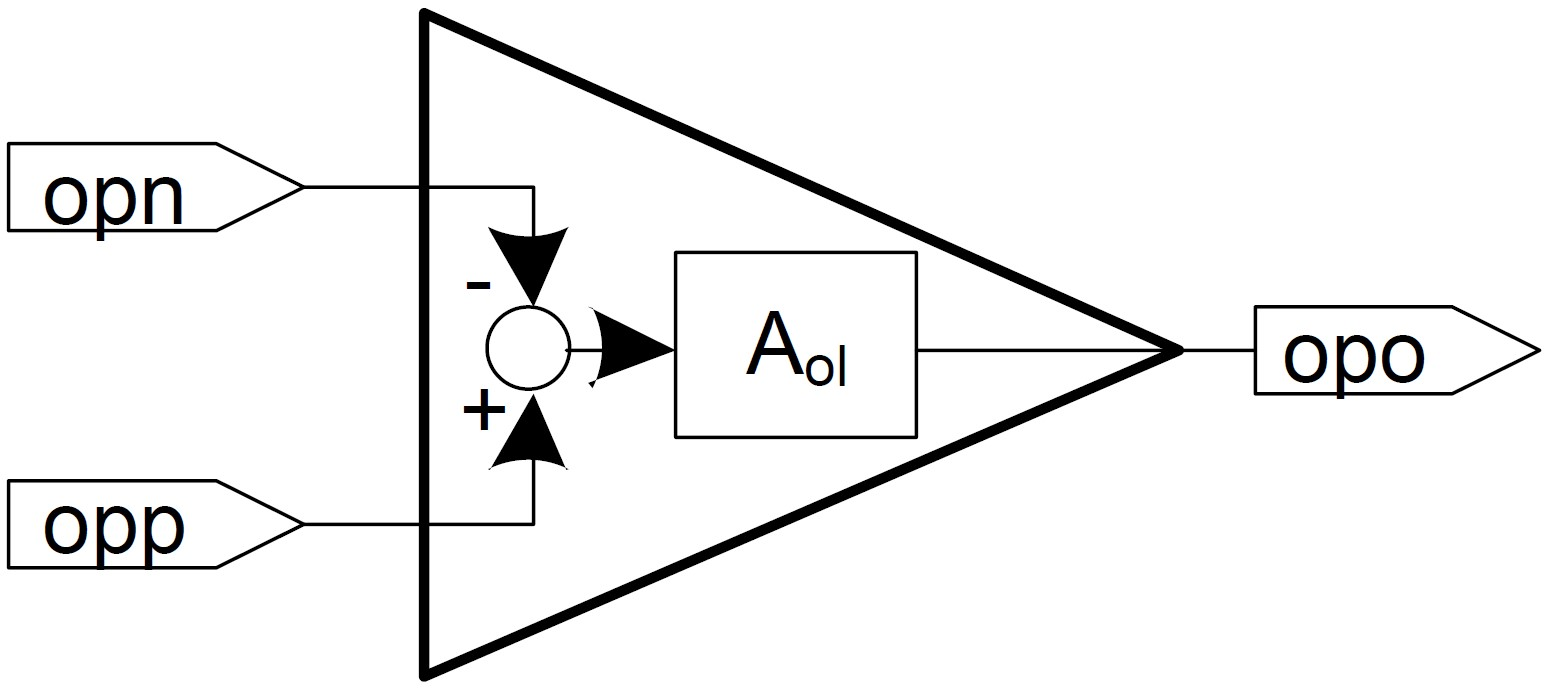
\includegraphics[width=0.8\columnwidth]{images/OPV_2.jpg}
\end{minipage}

\vspace{0.1cm}

\textbf{Idealer OpAmp:} \quad $A_{\rm ol} = \infty$ \quad $Z_{\rm in} = \infty$ ($I_{\rm opp} = I_{\rm opn} = 0$) \quad $Z_{\rm out} = 0$ \quad $V_{\rm os} = 0$

$$ \boxed{ V_{\rm out} = A_{\rm ol} \cdot (V_{\rm opp} + V_{\rm os} - V_{\rm opn}) } $$

\subsubsection*{Legende}
\begin{itemize}
	\item \textbf{$V_{\rm os}$ (Tensione di offset d'ingresso):} tensione parassita in serie al morsetto $+$. Viene amplificata come un segnale su $V_{\rm opp}$.
	\item \textbf{$A_{\rm ol}$ (Guadagno ad anello aperto):} guadagno differenziale interno. Ideale $= \infty$ (genera il cortocircuito virtuale).
	\item \textbf{$A_{\rm cl}$ (Guadagno ad anello chiuso):} guadagno effettivo del circuito con retroazione, $A_{\rm cl} = V_{\rm out}/V_{\rm in}$.
	\item \textbf{$V_{\rm AGND}$ ($= V_{\rm COM}$):} potenziale di riferimento (massa analogica).
\end{itemize}


\subsection{OpAmp als Verstärker}

\begin{itemize}
	\item \textbf{Rückkopplung auf negativen Eingang} \textrightarrow\ OpAmp stellt $V_{\rm out}$ so ein, dass \\
		$V_{\rm opn} = V_{\rm opp}$ \quad (\textbf{virtueller Kurzschluss}; liegt opp an AGND: opn = virtuelle Masse)
	\item $I_{\rm opn} = I_{\rm opp} = 0$ \textrightarrow\ Strom durch Eingangs-R = Strom durch Rückkopplungs-R
	\item Lineare Schaltung (solange nicht am Anschlag) \textrightarrow\ \textbf{Superposition}: \\
		jede Quelle einzeln, andere Spannungsquellen auf AGND setzen
	\item \cbl{Für $A_{\rm ol} \neq \infty$}: $V_{\rm opn}$ per Superposition aus $V_{\rm out}$ und den Eingängen ausdrücken, \\
		in Grundgleichung einsetzen und nach $V_{\rm out}$ auflösen
\end{itemize}

\myul{\textbf{Rückkopplungsfaktor und Closed-Loop-Gain}}

\vspace{0.1cm}

\begin{minipage}[c]{0.48\columnwidth}
	$$ \beta = \frac{V_{\rm opn}}{V_{\rm out}}\Bigg|_{\text{Eing. aus}} = \frac{R_1}{R_1 + R_2} $$
	\centering ($R_2$: Rückkopplung, $R_1$: nach AGND bzw. $V_{\rm in}$)
\end{minipage}
\hfill
\begin{minipage}[c]{0.48\columnwidth}
	Schleifenverstärkung: $\beta A_{\rm ol}$ \\
	Rauschverstärkung (Noise Gain): $\dfrac{1}{\beta} = 1 + \dfrac{R_2}{R_1}$
\end{minipage}

\vspace{0.1cm}

$$ \boxed{ A_{\rm cl} = A_{\rm ideal} \cdot \frac{\beta A_{\rm ol}}{1 + \beta A_{\rm ol}} \approx A_{\rm ideal} \left( 1 - \frac{1}{\beta A_{\rm ol}} \right) } $$
\centerline{rel. Fehler: $\varepsilon \approx \frac{1}{\beta A_{\rm ol}}$}

Nicht-invertierend: $A_{\rm ideal} = \frac{1}{\beta}$ \textrightarrow\ $A_{\rm cl} = \frac{A_{\rm ol}}{1 + \beta A_{\rm ol}}$ \qquad
Invertierend: $A_{\rm ideal} = -\frac{R_2}{R_1}$


\subsection{Grundschaltungen OpAmp}

\subsubsection{Nicht-Invertierender Verstärker}

\begin{minipage}[c]{0.4\columnwidth}
	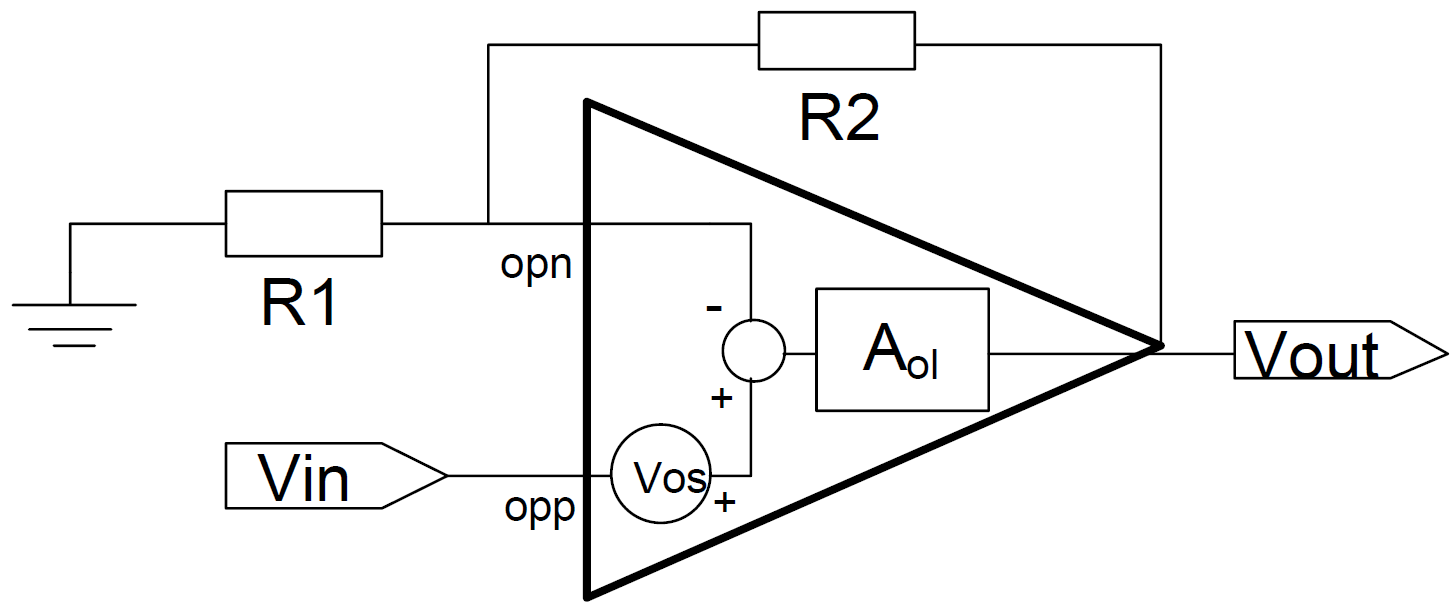
\includegraphics[width=\columnwidth]{images/nicht-invertierender_verstaerker_offset.png}
\end{minipage}
\hfill
\begin{minipage}[c]{0.58\columnwidth}
	\textbf{Spannungsteiler an opn:}
	$$ V_{\rm opn} = \frac{R_2}{R_1 + R_2} \cdot V_{\rm AGND} + \frac{R_1}{R_1 + R_2} \cdot V_{\rm out} $$
	\textbf{Gain:} \quad $\boxed{ A = 1 + \dfrac{R_2}{R_1} = \dfrac{1}{\beta} }$ \\[0.1cm]
	$Z_{\rm in} \approx \infty$, \quad gleichphasig ($0 \, \degree$)
\end{minipage}

\vspace{0.1cm}

\begin{minipage}[t]{0.5\columnwidth}
	\textbf{Real}

	\scalebox{0.8}{
	$ \boxed{ V_{\rm out} = \frac{A_{\rm ol}}{1 + \beta A_{\rm ol}} \Big[ V_{\rm in} + V_{\rm os} - \frac{R_2}{R_1 + R_2} V_{\rm AGND} \Big] } $}
\end{minipage}
\hfill
\begin{minipage}[t]{0.48\columnwidth}
	\textbf{Ideal}

	\scalebox{0.8}{
	$ \boxed{ V_{\rm out} = \Big(1 + \frac{R_2}{R_1}\Big)(V_{\rm in} + V_{\rm os}) - \frac{R_2}{R_1} V_{\rm AGND} } $}
\end{minipage}


\subsubsection{Invertierender Verstärker}

\begin{minipage}[c]{0.4\columnwidth}
	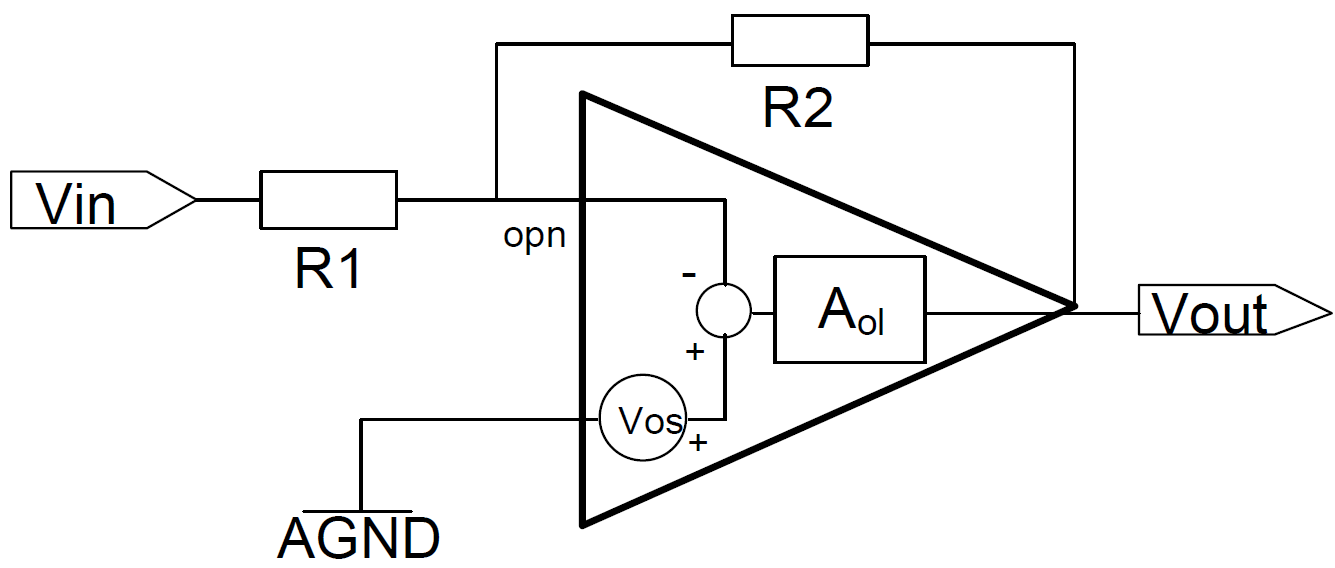
\includegraphics[width=0.9\columnwidth]{images/invertierender_verstaerker_offset.png}
\end{minipage}
\hfill
\begin{minipage}[c]{0.58\columnwidth}
	\textbf{Knoten opn} ($I_{\rm opn} = 0$, ideal $V_{\rm opn} = 0$):
	$$ \frac{V_{\rm in} - V_{\rm opn}}{R_1} = \frac{V_{\rm opn} - V_{\rm out}}{R_2} \;\Rightarrow\; V_{\rm out} = -\frac{R_2}{R_1} V_{\rm in} $$
	\textbf{Spannungsteiler an opn:}
	$$ V_{\rm opn} = \frac{R_2}{R_1 + R_2} \cdot V_{\rm in} + \frac{R_1}{R_1 + R_2} \cdot V_{\rm out} $$
\end{minipage}

\vspace{0.1cm}

\textbf{Gain:} \quad $\boxed{ A = -\dfrac{R_2}{R_1} }$ \qquad $Z_{\rm in} = R_1$, \quad gegenphasig ($180 \, \degree$), \quad Noise Gain $\frac{1}{\beta} = 1 + \frac{R_2}{R_1} \neq |A|$

\vspace{0.1cm}

\begin{minipage}[t]{0.5\columnwidth}
	\textbf{Real}

	\scalebox{0.8}{
	$ \boxed{ V_{\rm out} = \frac{A_{\rm ol}}{1 + \beta A_{\rm ol}} \Big[ V_{\rm AGND} + V_{\rm os} - \frac{R_2}{R_1 + R_2} V_{\rm in} \Big] } $}
\end{minipage}
\hfill
\begin{minipage}[t]{0.48\columnwidth}
	\textbf{Ideal}

	\scalebox{0.8}{
	$ \boxed{ V_{\rm out} = \Big(1 + \frac{R_2}{R_1}\Big)(V_{\rm AGND} + V_{\rm os}) - \frac{R_2}{R_1} V_{\rm in} } $}
\end{minipage}


\subsubsection{Invertierender Summierender Verstärker (Addierer)}

\begin{minipage}[c]{0.38\columnwidth}
	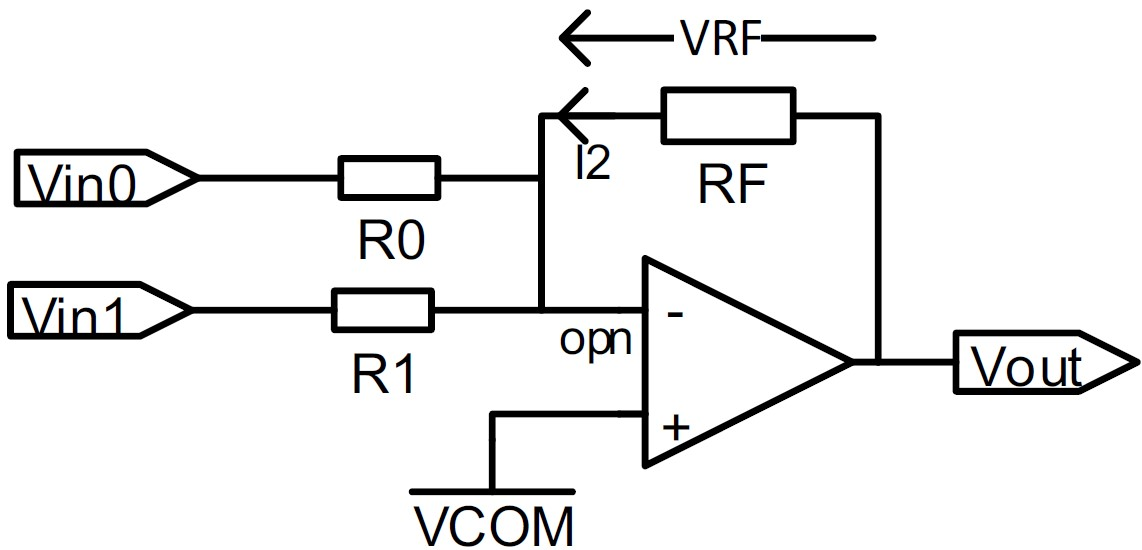
\includegraphics[width=\columnwidth]{images/invertierender_summierender_verstaerker.jpg}
\end{minipage}
\hfill
\begin{minipage}[c]{0.6\columnwidth}
	Knoten opn: \quad $I_2 = -I_0 - I_1$
	\[ I_0 = \frac{V_{\rm in0} - V_{\rm COM} - V_{\rm os}}{R_0} \qquad I_1 = \frac{V_{\rm in1} - V_{\rm COM} - V_{\rm os}}{R_1} \]
	\textbf{Gain pro Eingang:} \quad $\boxed{ A_i = -\dfrac{R_F}{R_i} }$ \\[0.1cm]
	opn = virtuelle Masse \textrightarrow\ Eingänge beeinflussen sich nicht
\end{minipage}

\vspace{0.1cm}

$$ \boxed{ V_{\rm out} = (V_{\rm COM} + V_{\rm os}) \cdot \Bigg( 1 + \frac{R_F}{R_0 || R_1} \Bigg) - R_F \cdot \Bigg( \frac{V_{\rm in0}}{R_0} + \frac{V_{\rm in1}}{R_1} \Bigg) } $$

Für $R_0 = R_1 = R$, $V_{\rm COM} = 0$: \quad $V_{\rm out} = -\frac{R_F}{R} \, (V_{\rm in0} + V_{\rm in1})$


\subsubsection{Buffer (Spannungsfolger)}

\begin{minipage}[c]{0.48\columnwidth}
	\begin{center}
		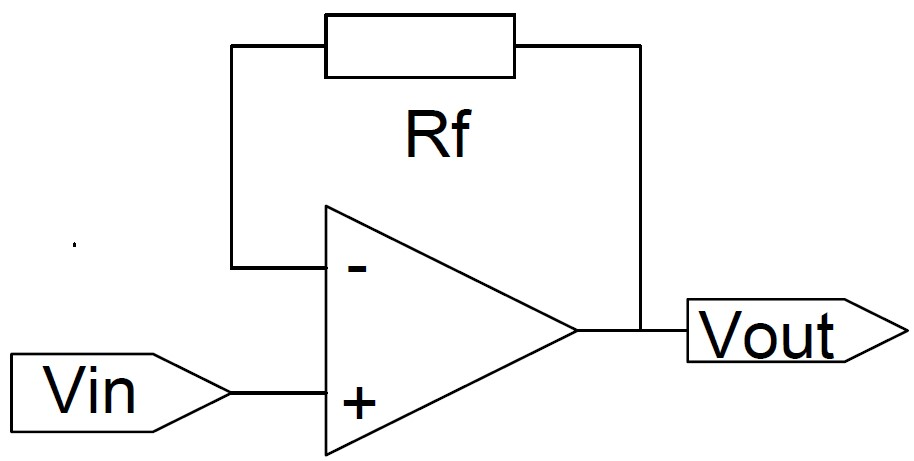
\includegraphics[width=0.65\columnwidth]{images/buffer_1.jpg}
	\end{center}
\end{minipage}
\hfill
\begin{minipage}[c]{0.48\columnwidth}
	\begin{center}
		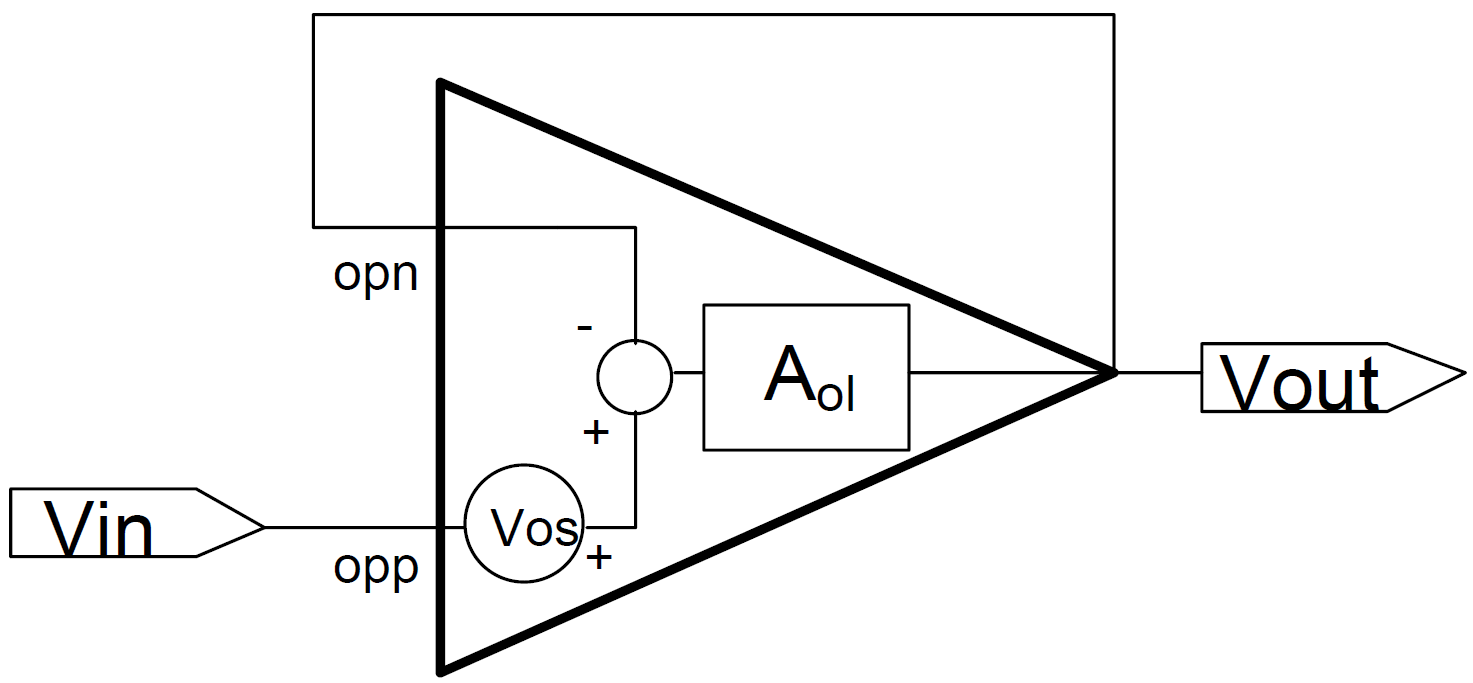
\includegraphics[width=0.7\columnwidth]{images/buffer_offset.png}
	\end{center}
\end{minipage}

\begin{minipage}[c]{0.48\columnwidth}
	\begin{itemize}
		\item \textbf{Gain} $A = 1$, \; $\beta = 1$ ($V_{\rm opn} = V_{\rm out}$)
		\item $Z_{\rm in} \approx \infty$ \textrightarrow\ keine Belastung an $V_{\rm in}$
		\item $Z_{\rm out} \approx 0$ \textrightarrow\ Impedanzwandler
	\end{itemize}
\end{minipage}
\hfill
\begin{minipage}[c]{0.48\columnwidth}
	\textbf{Real:} \quad $\boxed{ V_{\rm out} = \dfrac{A_{\rm ol}}{1 + A_{\rm ol}} (V_{\rm in} + V_{\rm os}) }$ \\[0.15cm]
	\textbf{Ideal:} \quad $\boxed{ V_{\rm out} = V_{\rm in} + V_{\rm os} }$ \\[0.1cm]
	$\frac{V_{\rm out}}{V_{\rm in}} \approx 1 - \frac{1}{A_{\rm ol}}$
\end{minipage}


\subsubsection*{Übersicht Grundschaltungen (ideal)}

\begin{center}
\renewcommand{\arraystretch}{1.4}
\begin{tabular}{l|c|c|c}
	\textbf{Schaltung} 	& \textbf{Gain $A$} 					& \textbf{$Z_{\rm in}$} 	& \textbf{Phase} \\ \hline
	Buffer				& $1$									& $\infty$					& $0 \, \degree$ \\
	Nicht-invertierend	& $1 + \frac{R_2}{R_1}$ 				& $\infty$					& $0 \, \degree$ \\
	Invertierend		& $-\frac{R_2}{R_1}$ 					& $R_1$						& $180 \, \degree$ \\
	Addierer			& $-\frac{R_F}{R_i}$ pro Eingang		& $R_i$						& $180 \, \degree$ \\
	Differenzverstärker	& $\frac{R_4}{R_3}$ auf $V_{\rm in1} - V_{\rm in2}$ & endlich		& -- \\
	Instrumentenverst.	& $\frac{R_4}{R_3}\big(1 + \frac{R_{f1} + R_{f2}}{R_g}\big)$ & $\infty$ & --
\end{tabular}
\end{center}


\subsection{Analoge Rechenschaltungen mit OpAmps}

\subsubsection{Differenzverstärker (Gewichteter Subtrahierer)}

\begin{minipage}[c]{0.4\columnwidth}
	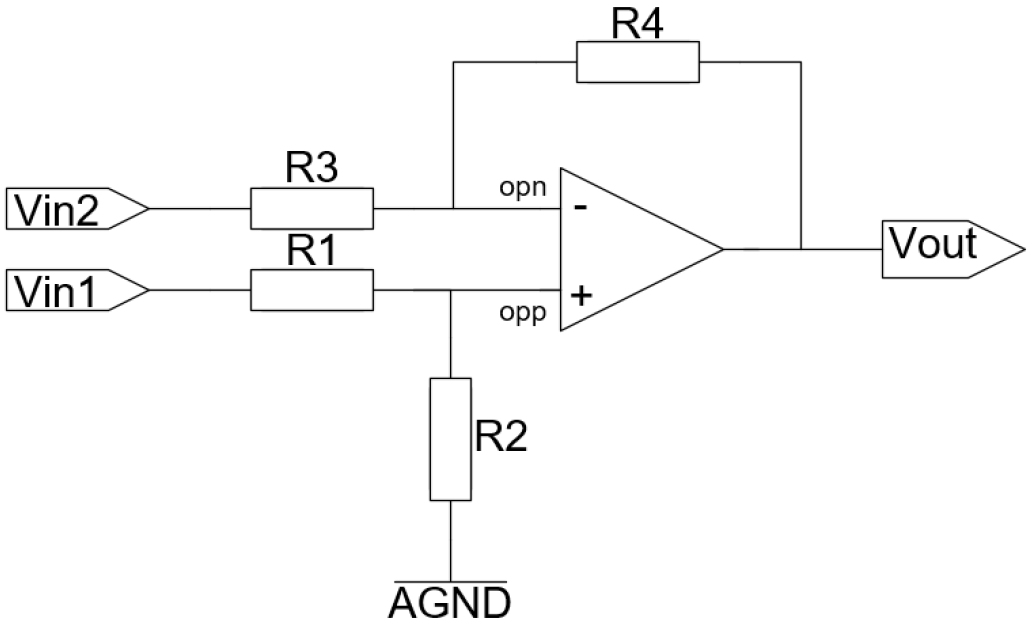
\includegraphics[width=\columnwidth]{images/differenzverstärker.png}
\end{minipage}
\hfill
\begin{minipage}[c]{0.58\columnwidth}
	\textbf{Superposition:} \\
	nur $V_{\rm in2}$ (oben): invertierend \textrightarrow\ $-\frac{R_4}{R_3}$ \\
	nur $V_{\rm opp}$ (unten): nicht-invertierend \textrightarrow\ $1 + \frac{R_4}{R_3}$
	$$ V_{\rm out} = \frac{R_3 + R_4}{R_3} \cdot V_{\rm opp} - \frac{R_4}{R_3} \cdot V_{\rm in2} $$
	Spannungsteiler: $V_{\rm opp} = \frac{R_1}{R_1 + R_2} V_{\rm AGND} + \frac{R_2}{R_1 + R_2} V_{\rm in1}$
\end{minipage}

$$ \boxed{ V_{\rm out} = \frac{R_3 + R_4}{R_3} \cdot \Bigg( \frac{R_1}{R_1 + R_2} \cdot V_{\rm AGND} + \frac{R_2}{R_1 + R_2} \cdot V_{\rm in1} \Bigg) - \frac{R_4}{R_3} \cdot V_{\rm in2} } $$
$$ \boxed{ \text{Für } R_1 = R_3, \, R_2 = R_4: \quad V_{\rm out} = V_{\rm AGND} + \frac{R_4}{R_3} \cdot ( V_{\rm in1} - V_{\rm in2}) } $$

\textbf{Gain:} \quad Differenz $A_D = \frac{R_4}{R_3}$, \quad $A_{\rm AGND} = 1$, \quad Gleichtakt $A_{\rm CM} = 0$ \\
Nachteile: R-Toleranzen \textrightarrow\ $A_{\rm CM} \neq 0$ (CMRR endlich); \; $Z_{\rm in}$ endlich \textrightarrow\ Instrumentenverstärker


\subsubsection{Instrumentenverstärker}

1. Stufe: OP1 und OP2 nicht-invertierend mit gemeinsamem $R_g$, 2. Stufe: Differenzverstärker

\begin{minipage}[c]{0.5\columnwidth}
	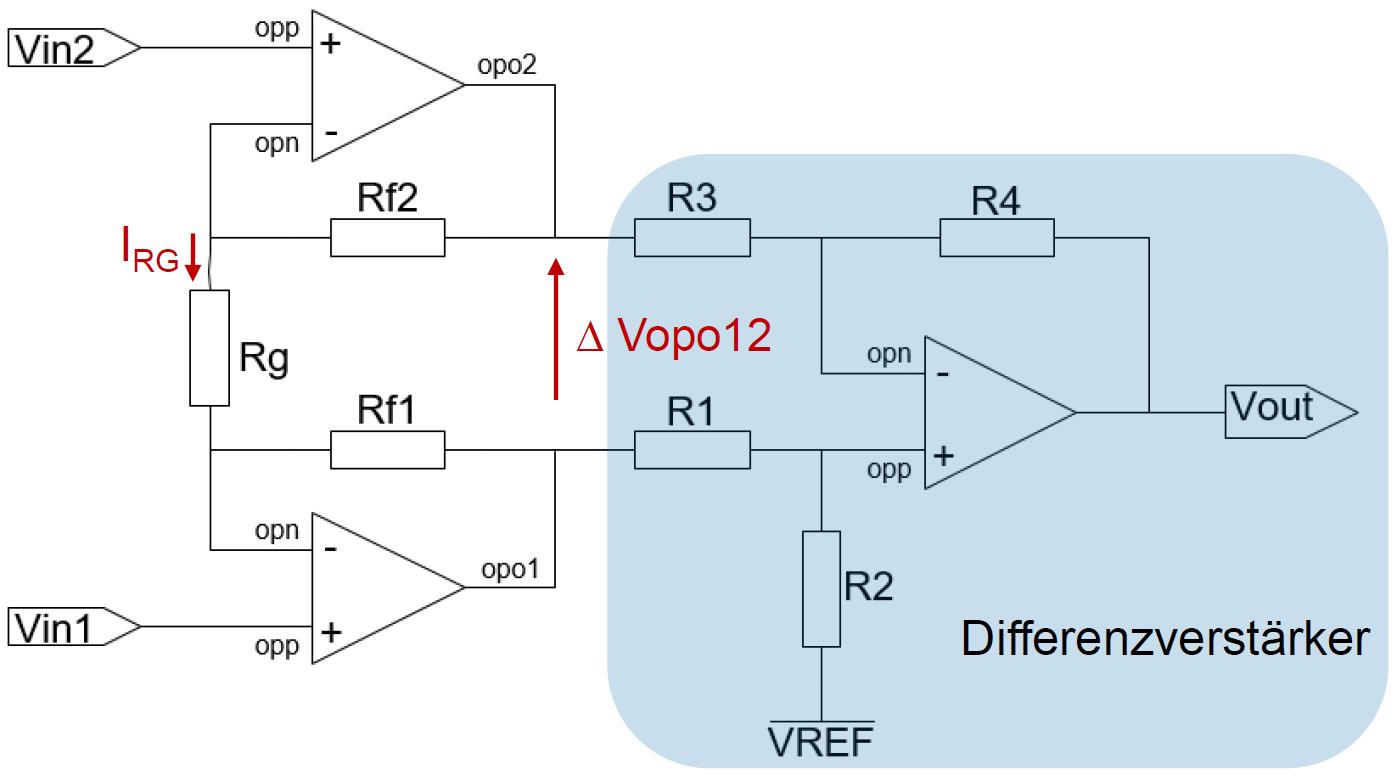
\includegraphics[width=\columnwidth]{images/instrumentenverstaerker.png}
\end{minipage}
\hfill
\begin{minipage}[c]{0.48\columnwidth}
	$$ I_{\rm Rg} = \frac{V_{\rm in2} - V_{\rm in1}}{R_g} $$
	$$ V_{\rm opo2} = V_{\rm in2} + \frac{R_{f2}}{R_g} \cdot (V_{\rm in2} - V_{\rm in1}) $$
	$$ V_{\rm opo1} = V_{\rm in1} + \frac{R_{f1}}{R_g} \cdot (V_{\rm in1} - V_{\rm in2}) $$
\end{minipage}

\[ \boxed{ \Delta V_{\rm opo} = V_{\rm opo1} - V_{\rm opo2} = \Bigg( 1 + \frac{R_{f1} + R_{f2}}{R_g} \Bigg) \cdot (V_{\rm in1} - V_{\rm in2}) } \]
\[ \boxed{ \text{Für } R_1 = R_3, \, R_2 = R_4: \quad V_{\rm out} = V_{\rm REF} + \frac{R_4}{R_3} \cdot \Bigg( 1 + \frac{R_{f1} + R_{f2}}{R_g} \Bigg) \cdot (V_{\rm in1} - V_{\rm in2}) } \]

\textbf{Gain:} \quad $A = \frac{R_4}{R_3} \Big( 1 + \frac{R_{f1} + R_{f2}}{R_g} \Big)$ \quad ($R_{f1} = R_{f2} = R_f$: $A = \frac{R_4}{R_3} \big( 1 + \frac{2 R_f}{R_g} \big)$)
\begin{itemize}
	\item Gain mit \textbf{einem} Widerstand $R_g$ einstellbar
	\item $Z_{\rm in} \approx \infty$ an beiden Eingängen
	\item Gleichtakt: $I_{\rm Rg} = 0$ \textrightarrow\ 1. Stufe hat Gain 1 für Gleichtakt \textrightarrow\ hohe CMRR
\end{itemize}


\subsection{Mehrstufige Verstärker}

\begin{center}
	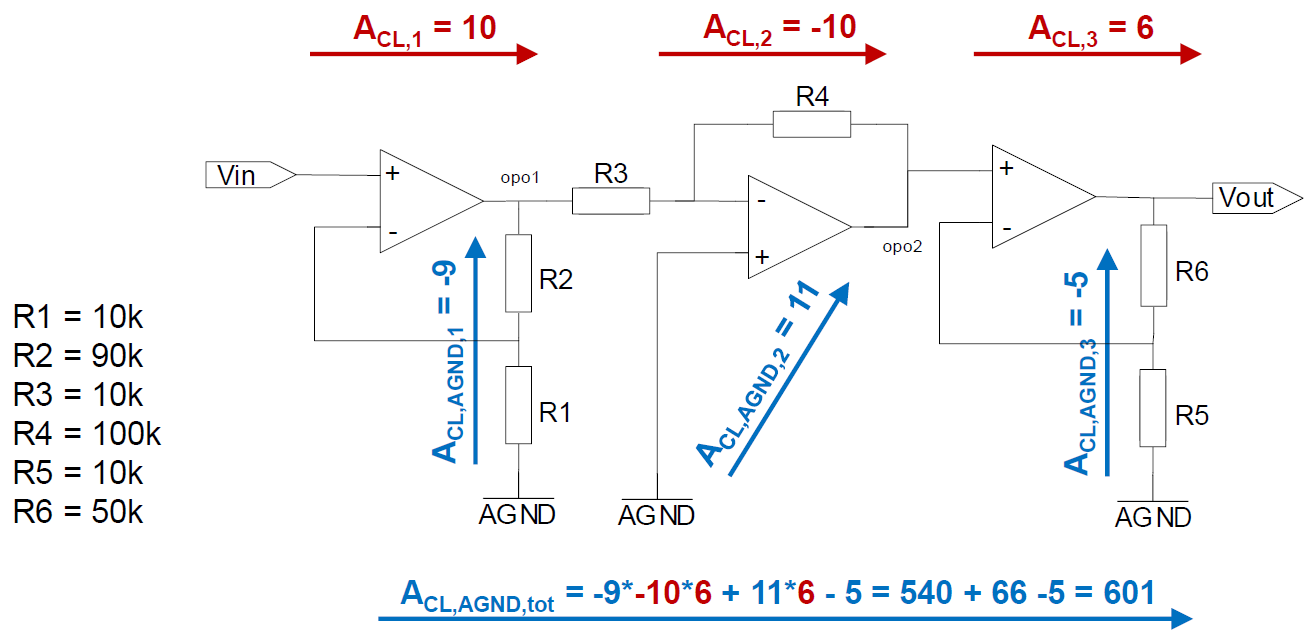
\includegraphics[width=0.85\columnwidth]{images/mehrstufige_verstaerker.png}
\end{center}

\begin{itemize}
	\item Gesamt-Gain: \quad $A_{\rm tot} = A_1 \cdot A_2 \cdot A_3$ \qquad bzw. \quad $A_{\rm tot,dB} = A_{\rm dB1} + A_{\rm dB2} + A_{\rm dB3}$
	\item Für $V_{\rm AGND} \neq 0 \, \volt$: Superposition, AGND als Quelle, Signaleingang 'ausschalten'
	\item AGND-Gain einer Stufe: \quad $A_{\rm AGND} = 1 - A$ \qquad (z.B. $A = 10$ \textrightarrow\ $-9$; \; $A = -10$ \textrightarrow\ $11$)
\end{itemize}

$$ \boxed{ V_{\rm out} = A_{\rm tot} \cdot V_{\rm in} + (1 - A_{\rm tot}) \cdot V_{\rm AGND} } $$
$$ \text{bzw.} \quad V_{\rm out} - V_{\rm AGND} = A_{\rm tot} \, (V_{\rm in} - V_{\rm AGND}) $$

Bild: $A_{\rm tot} = 10 \cdot (-10) \cdot 6 = -600$ \textrightarrow\ $A_{\rm AGND,tot} = 1 - (-600) = 601$ \; \checkmark


\subsection{Gesteuerte Quellen}

\subsubsection{Stromgesteuerte Stromquellen}

\begin{minipage}[c]{0.4\columnwidth}
	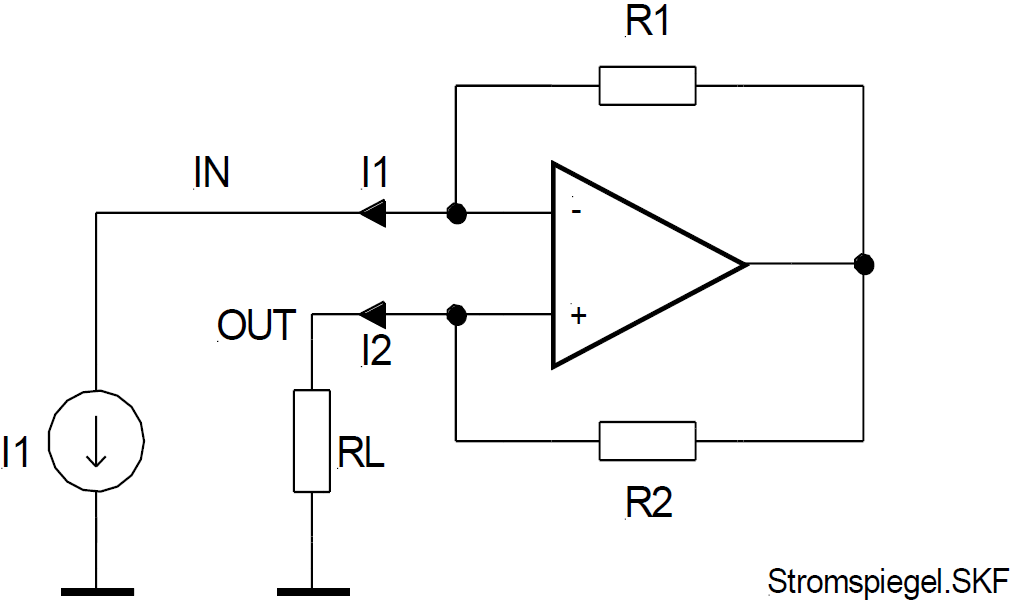
\includegraphics[width=\columnwidth]{images/stromspiegel_OPV.png}
\end{minipage}
\hfill
\begin{minipage}[c]{0.48\columnwidth}
	$$ V_{R1} = V_{R2} \qquad R_1 \, I_1 = R_2 \, I_2 $$
	\textbf{Stromverstärkung:}
	$$ \boxed{ A_i = \frac{I_2}{I_1} = \frac{R_1}{R_2} } $$
\end{minipage}


\subsubsection{Spannungsgesteuerte Stromquellen}

Strom unabhängig von der Last $R_L$, \quad Transkonduktanz $g = \frac{I_L}{V_{\rm in}}$

\begin{minipage}[c]{0.48\columnwidth}
	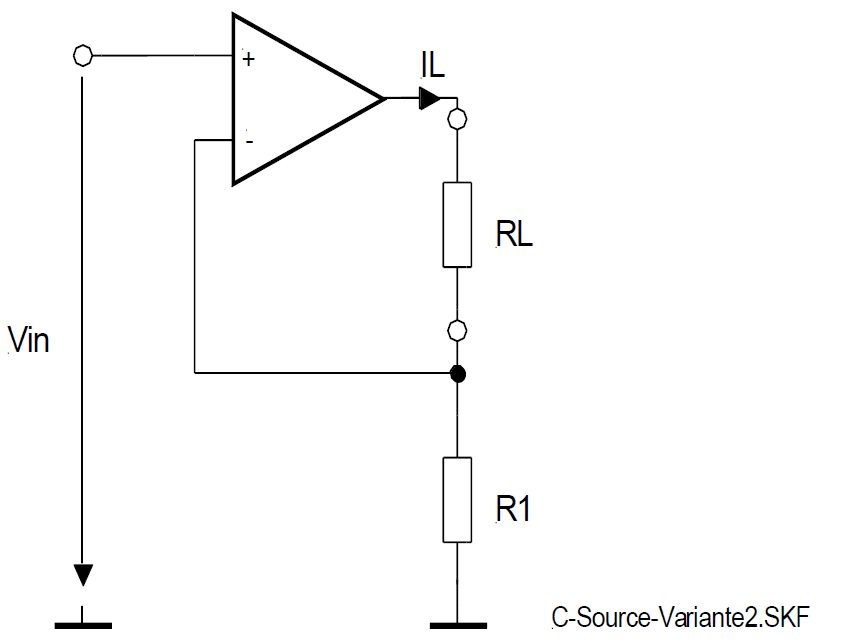
\includegraphics[width=\columnwidth]{images/spannungsgesteuerte_stromquelle_V1.png}
	$$ \boxed{ I_L = \frac{V_{\rm in}}{R_1} } $$
	Nachteil: Last muss 'floating' sein
\end{minipage}
\hfill
\begin{minipage}[c]{0.48\columnwidth}
	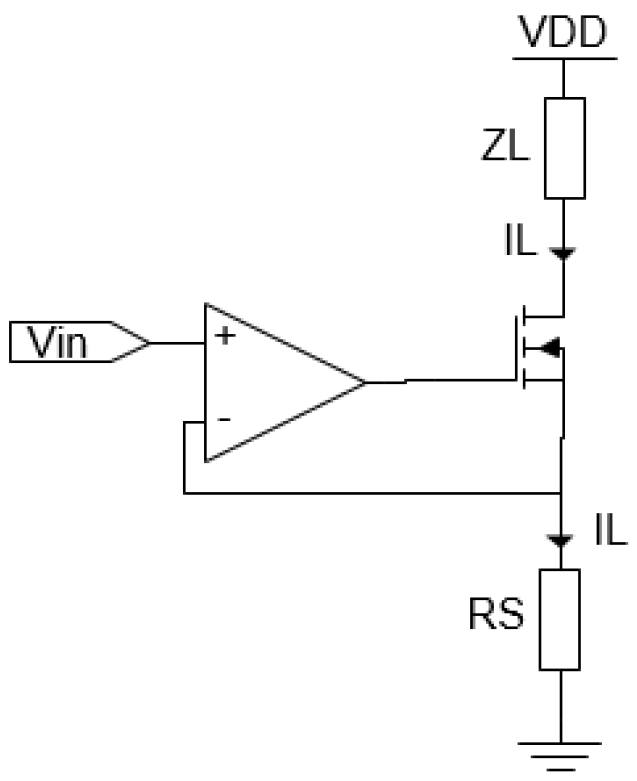
\includegraphics[width=0.6\columnwidth]{images/spannungsgesteuerte_stromquelle_V2.png}
	$$ \boxed{ I_L = \frac{V_{\rm in}}{R_s} } $$
	Last gegen VDD, Transistor liefert Strom
\end{minipage}


\subsection{Einfache Filterschaltungen mit OpAmps}

Alle Filter = invertierender Verstärker mit Impedanzen: \quad $\boxed{ H(j\omega) = -\dfrac{Z_f}{Z_{\rm in}} }$ \quad $Z_C = \dfrac{1}{j \omega C}$

\subsubsection{Integratoren}

\begin{tabular}{ll}
	RL-Integrator:	& Spulen sind nichtideal und teuer, erzeugen oft Oszillationen \\
	RC-Integrator: 	& fast immer für aktive Filter verwendet
\end{tabular}

\vspace{0.2cm}

\begin{minipage}[c]{0.4\columnwidth}
	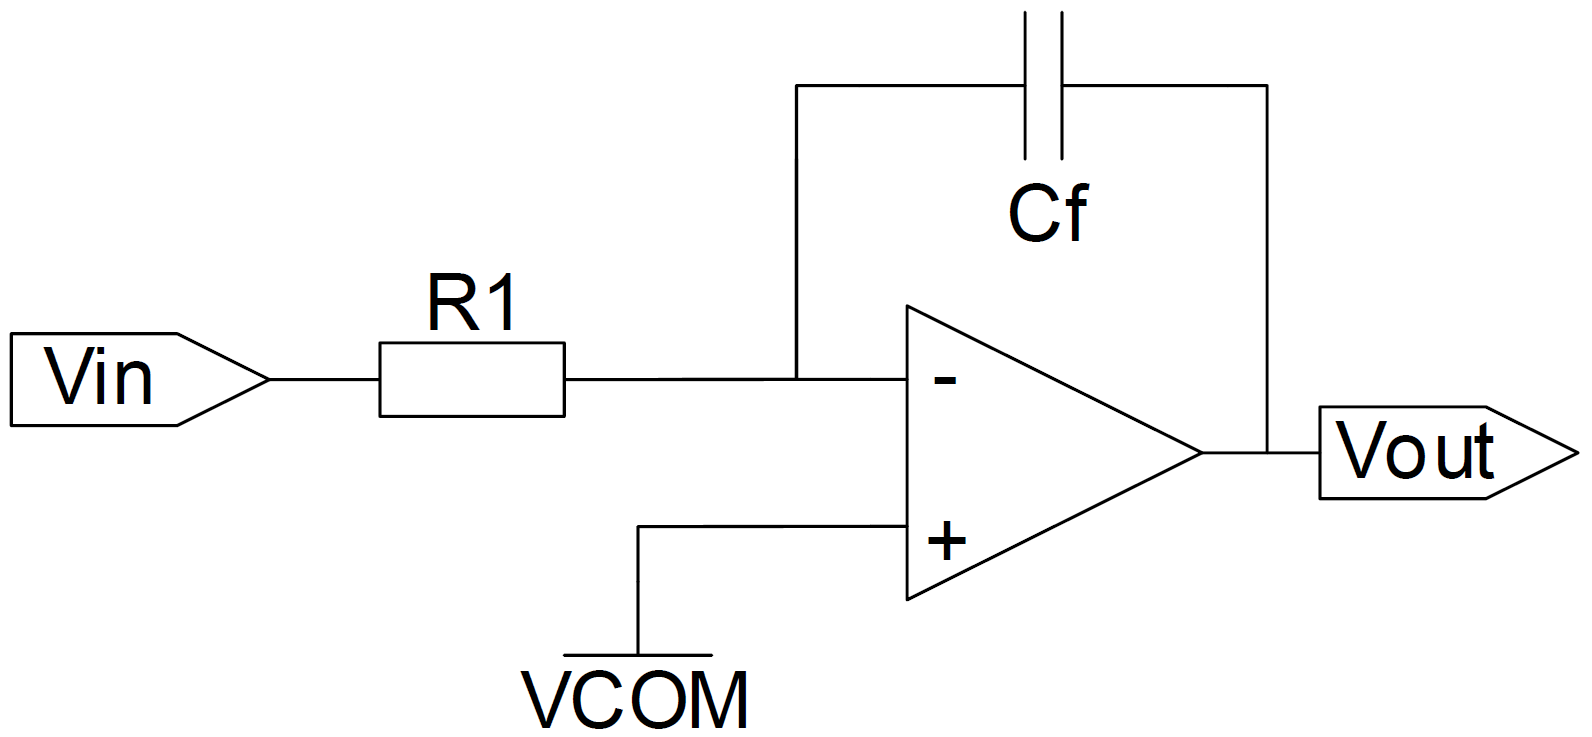
\includegraphics[width=\columnwidth]{images/integrator.png}
\end{minipage}
\hfill
\begin{minipage}[c]{0.58\columnwidth}
	$I = \frac{V_{\rm in}}{R_1}$ fliesst ganz in $C_f$, \; $V_{\rm out} = -V_{C}$
	$$ \boxed{ V_{\rm out}(t) = - \frac{1}{R_1 C_f} \int\limits_0^t V_{\rm in}(\tau) \, \diff \tau + V_{\rm out}(0) } $$
	$$ V_{\rm out}(t) = - \frac{1}{C_f} \int\limits_0^t I_{C_f}(\tau) \, \diff \tau + V_{\rm out}(0) $$
\end{minipage}

\vspace{0.1cm}

\begin{minipage}[c]{0.5\columnwidth}
	$$ \boxed{ H(j\omega) = -\frac{1}{j \omega R_1 C_f} } \qquad |H| = \frac{1}{\omega R_1 C_f} $$
\end{minipage}
\hfill
\begin{minipage}[c]{0.48\columnwidth}
	$-20 \, \deci \bel$/Dek, \; Phase $+90 \, \degree$ \\
	$|H| = 1$ bei $f_0 = \frac{1}{2 \pi R_1 C_f}$
\end{minipage}

\begin{itemize}
	\item Konstante \textrightarrow\ Rampe, \; Rechteck \textrightarrow\ Dreieck, \; Sinus \textrightarrow\ Cosinus
	\item Problem: Gain bei DC $= \infty$ \textrightarrow\ $V_{\rm os}$, $I_B$ werden aufintegriert \textrightarrow\ Sättigung \\
		Lösung: $R_f$ parallel zu $C_f$ \textrightarrow\ Tiefpass
	\item Mit $V_{\rm COM} \neq 0$: \; $V_{\rm out} = V_{\rm COM} - \frac{1}{R_1 C_f} \int (V_{\rm in} - V_{\rm COM}) \, \diff \tau$
\end{itemize}


\subsubsection{Differenzierer}

\begin{minipage}[c]{0.4\columnwidth}
	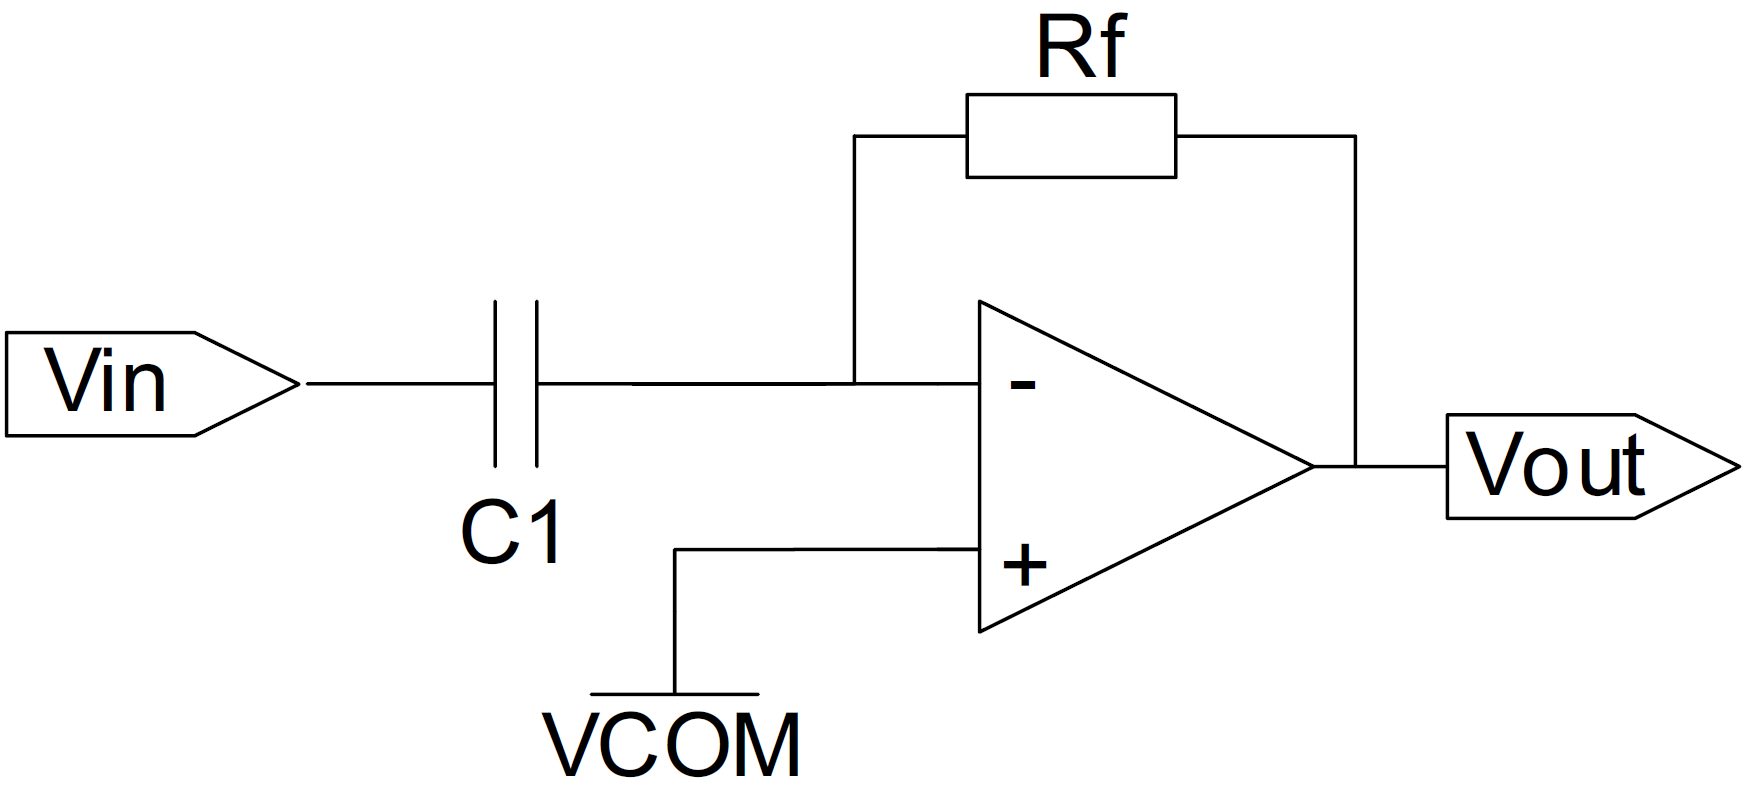
\includegraphics[width=\columnwidth]{images/differenzierer.png}
\end{minipage}
\hfill
\begin{minipage}[c]{0.58\columnwidth}
	$$ i_C = C_1 \frac{\diff V_{\rm in}}{\diff t} \qquad \boxed{ V_{\rm out} = - R_f C_1 \frac{\diff V_{\rm in}}{\diff t} } $$
	$$ \boxed{ H(j\omega) = -j \omega R_f C_1 } \qquad |H| = \omega R_f C_1 $$
	$+20 \, \deci \bel$/Dek, \; $|H| = 1$ bei $f_0 = \frac{1}{2 \pi R_f C_1}$
\end{minipage}

\vspace{0.1cm}

\myul{\textbf{Differenzierer im Frequenzbereich}}

\begin{itemize}
	\item Hohe Frequenzen werden mehr verstärkt (auch Rauschen!)
	\item Rückkopplungsfunktion ist Tiefpass, realer OpAmp bildet auch Tiefpass
	\item Beide Tiefpässe zusammen $180 \, \degree$ Phasenschiebung \textrightarrow\ Mitkopplung \textrightarrow\ Schwingung
	\item Kleines $C$ parallel zu $R_f$ unterdrückt Schwingungen
\end{itemize}


\subsubsection{Tiefpass}

\begin{minipage}[c]{0.4\columnwidth}
	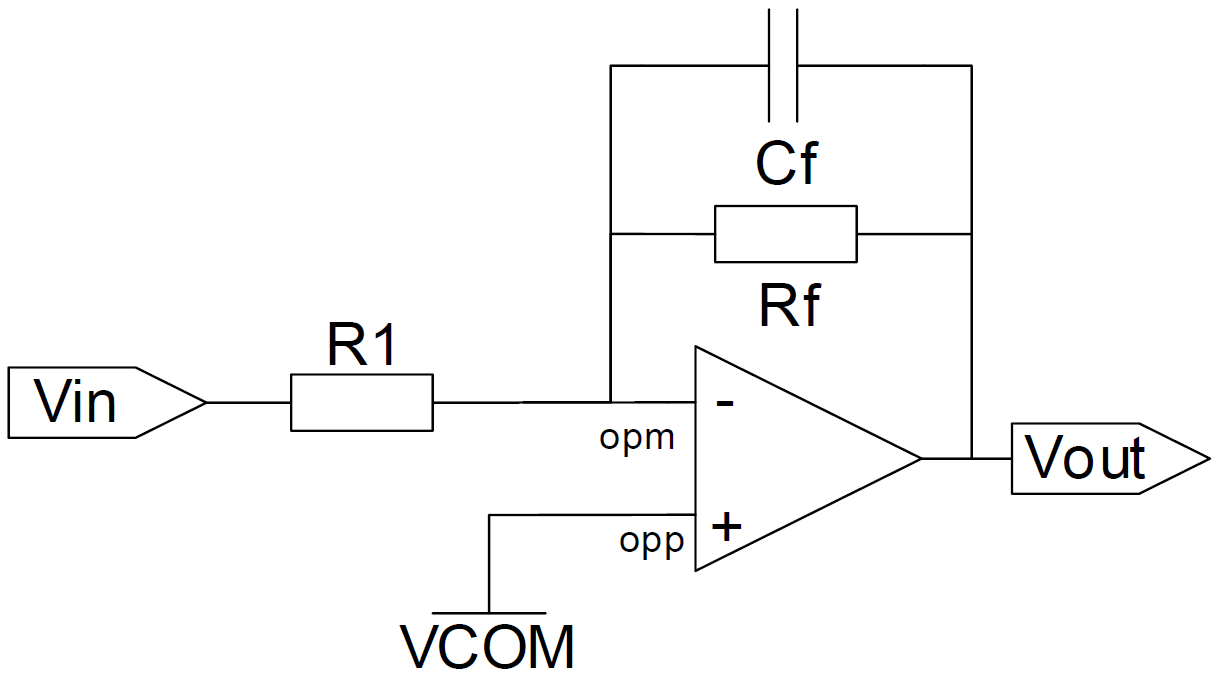
\includegraphics[width=\columnwidth]{images/tiefpass.png}
\end{minipage}
\hfill
\begin{minipage}[c]{0.58\columnwidth}
	\begin{tabular}{ll}
		\cbl{Tiefe $f$}:  	& $C_f$ offen \textrightarrow\ invertierend \\
		\cgn{Hohe $f$}:		& Integrator, $-20 \, \deci \bel$/Dek
	\end{tabular}

	$$ \boxed{ H(j\omega) = -\frac{R_f}{R_1} \cdot \frac{1}{1 + j \omega R_f C_f} } $$
	$$ \cbl{ \boxed{ A_{\rm DC} = - \frac{R_f}{R_1} } } \qquad \cgn{ \boxed{ f_g = \frac{1}{2 \pi R_f C_f} } } $$
\end{minipage}


\subsubsection{Bandpass}

\begin{minipage}[c]{0.48\columnwidth}
	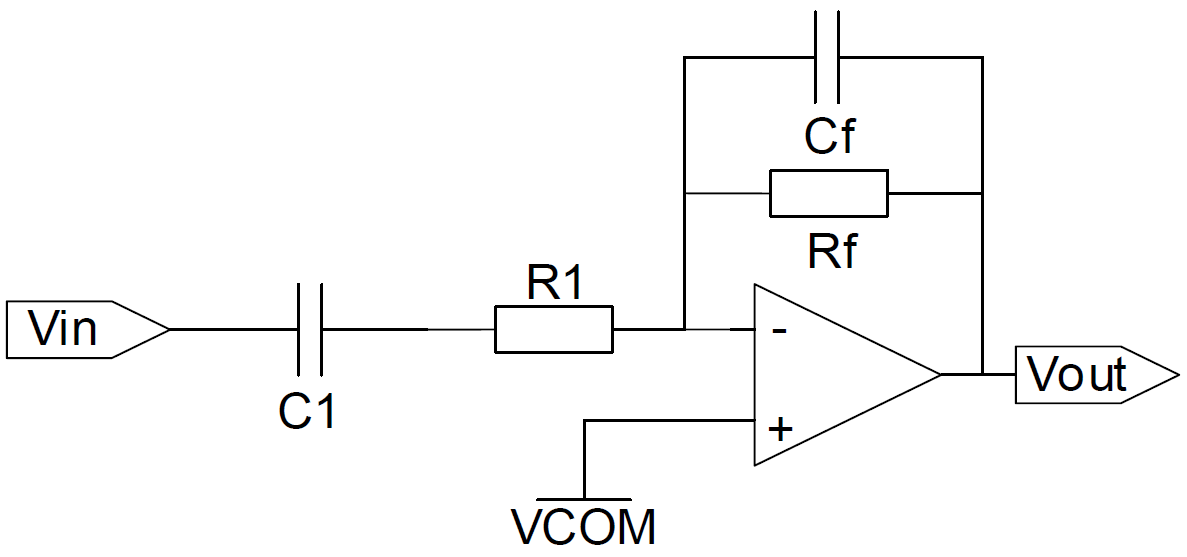
\includegraphics[width=\columnwidth]{images/bandpass.png}
\end{minipage}
\hfill
\begin{minipage}[c]{0.48\columnwidth}
	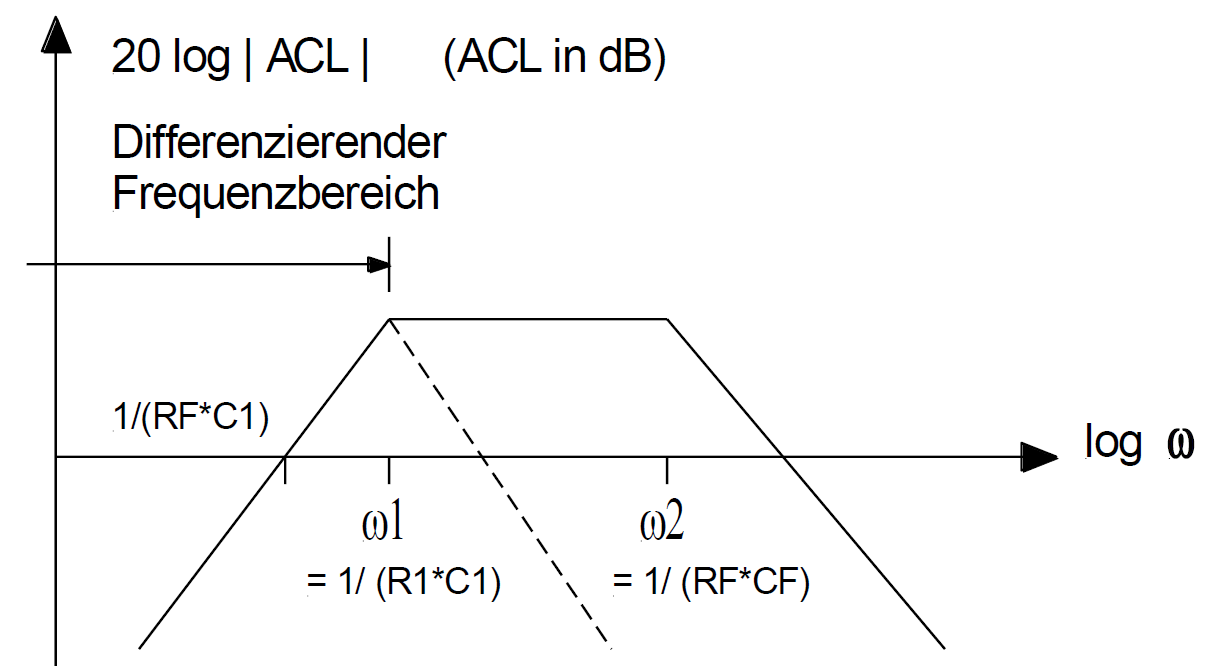
\includegraphics[width=\columnwidth]{images/bandpass_amplitudengang.png}
\end{minipage}

\vspace{0.1cm}

\begin{minipage}[c]{0.48\columnwidth}
	\begin{tabular}{ll}
		$C_1$ & sperrt tiefe $f$ (Hochpass) \\
		$R_1$ & limitiert Eingangsstrom \\
		$C_f$ & limitiert $V_{\rm out}$ bei hohen $f$
	\end{tabular}
\end{minipage}
\hfill
\begin{minipage}[c]{0.48\columnwidth}
	$$ f_u = \frac{1}{2 \pi R_1 C_1} \qquad f_o = \frac{1}{2 \pi R_f C_f} $$
	Durchlassbereich ($f_u \ll f \ll f_o$): \; $\boxed{ A = -\dfrac{R_f}{R_1} }$
\end{minipage}


\subsubsection{Allpass}

\begin{itemize}
	\item Betrag der Verstärkung $= 1$ für alle $f$
	\item Phase ändert mit der Frequenz von $180 \, \degree$ ($-V_{\rm in}$) auf $0 \, \degree$ ($+V_{\rm in}$)
\end{itemize}

\begin{minipage}[c]{0.4\columnwidth}
	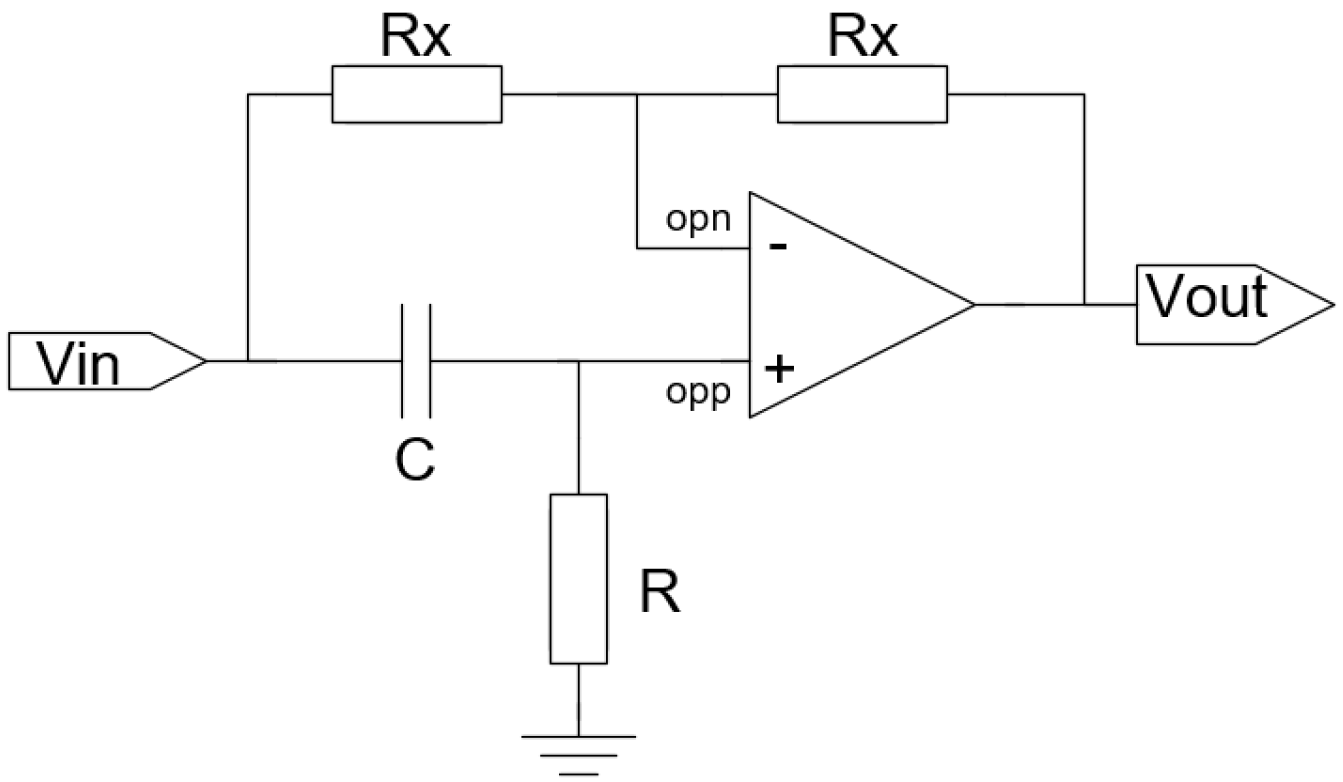
\includegraphics[width=\columnwidth]{images/allpass.png}
\end{minipage}
\hfill
\begin{minipage}[c]{0.58\columnwidth}
	\begin{tabular}{ll}
		\cbl{tiefe $f$}:	& $C$ sperrt, $V_{\rm opp} = 0$ \\
		\cgn{hohe $f$}: 	& $C$ Kurzschluss, $I_{R_x} = 0$
	\end{tabular}

	$$ \cbl{ \boxed{ V_{\rm out} = - \frac{R_x}{R_x} \cdot V_{\rm in} = - V_{\rm in} } } \qquad
	   \cgn{ \boxed{ V_{\rm out} = V_{\rm in} } } $$
\end{minipage}

$$ \boxed{ H(j\omega) = -\frac{1 - j \omega R C}{1 + j \omega R C} } \qquad |H| = 1 $$
$$ \varphi = 180 \, \degree - 2 \arctan(\omega R C) \qquad (90 \, \degree \text{ bei } f = \tfrac{1}{2 \pi R C}) $$


\subsection{Nichtidealitäten von OpAmps}

\subsubsection{Endliche Verstärkung $A_{\rm ol}$}

$$ V_d = V_{\rm opp} - V_{\rm opn} = \frac{V_{\rm out}}{A_{\rm ol}} \neq 0 \qquad \text{\textrightarrow\ Gain-Fehler } \varepsilon \approx \frac{1}{\beta A_{\rm ol}} $$

\begin{minipage}[c]{0.48\columnwidth}
	\textbf{Nicht-invertierend / Buffer:}
	$$ A_{\rm cl} = \frac{A_{\rm ol}}{1 + \beta A_{\rm ol}} \approx \frac{1}{\beta} \left(1 - \frac{1}{\beta A_{\rm ol}}\right) $$
\end{minipage}
\hfill
\begin{minipage}[c]{0.48\columnwidth}
	\textbf{Invertierend:}
	$$ A_{\rm cl} = -\frac{R_2}{R_1} \cdot \frac{\beta A_{\rm ol}}{1 + \beta A_{\rm ol}} \approx -\frac{R_2}{R_1} \left(1 - \frac{1}{\beta A_{\rm ol}}\right) $$
\end{minipage}

\subsubsection{Offset-Spannung $V_{\rm os}$}

Wirkt wie Quelle am +-Eingang \textrightarrow\ wird mit der \textbf{Noise Gain} verstärkt (auch beim invertierenden Verstärker):
$$ \boxed{ V_{\rm out,os} = V_{\rm os} \cdot \Big(1 + \frac{R_2}{R_1}\Big) = \frac{V_{\rm os}}{\beta} } $$

\subsubsection{Eingangsstromfehler - Bias-Strom $\rm{I_B}$}

\begin{minipage}[c]{0.48\columnwidth}
	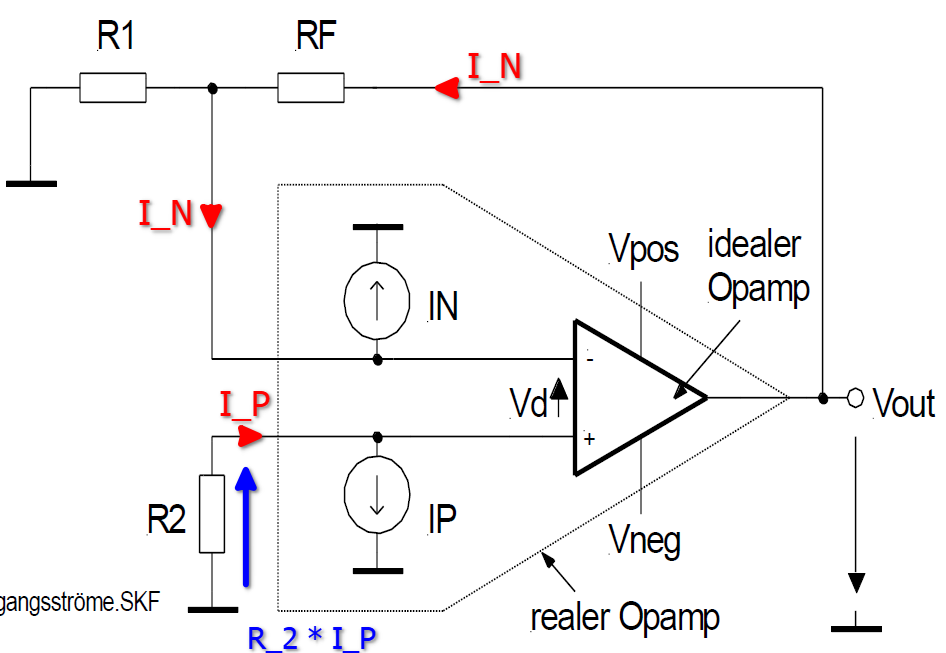
\includegraphics[width=\columnwidth]{images/bias-strom_grafik.png}
\end{minipage}
\hfill
\begin{minipage}[c]{0.48\columnwidth}
	Modellierung durch Stromquellen $I_P$, $I_N$

	\vspace{0.2cm}

	$V_{\rm outE}$: Fehlerspannung aufgrund von $I_P$, $I_N$

	$$ I_B = \frac{I_P + I_N}{2} $$
\end{minipage}

\vspace{0.2cm}
$$ \boxed{ V_{\rm outE} = V_{\rm outE(N)} + V_{\rm outE(P)} = I_N \, R_F - I_P \, R_2 \Bigg( \frac{R_F + R_1}{R_1} \Bigg) } $$

\textbf{Kompensation} ($I_N = I_P$, $V_{\rm outE} \overset{!}{=} 0$):
$$ R_F = R_2 \, \Bigg( \frac{R_F + R_1}{R_1} \Bigg) \quad \Rightarrow \quad \boxed{ R_2 = \frac{R_F \cdot R_1}{R_F + R_1} = R_F || R_1 } $$
\textrightarrow\ beide Eingänge sehen den gleichen Widerstand

\vspace{0.1cm}

\myul{\textbf{Bias-Strom-Kompensation mittels $\bm{R_2}$}}

\vspace{0.1cm}

\begin{minipage}[b]{0.3\columnwidth}
	\begin{center}
		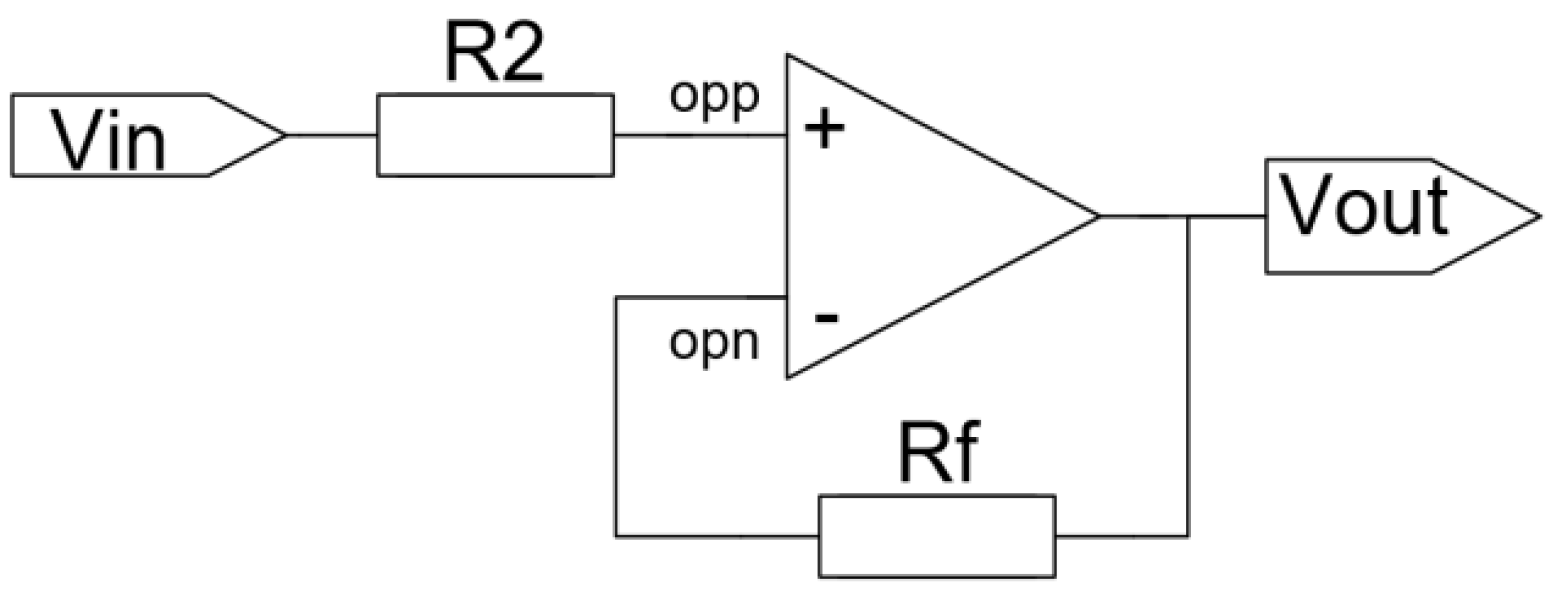
\includegraphics[width=\columnwidth]{images/kompensation_bias-strom_1.png}
		$$ R_2 = R_F $$
	\end{center}
\end{minipage}
\hfill
\begin{minipage}[b]{0.3\columnwidth}
	\begin{center}
		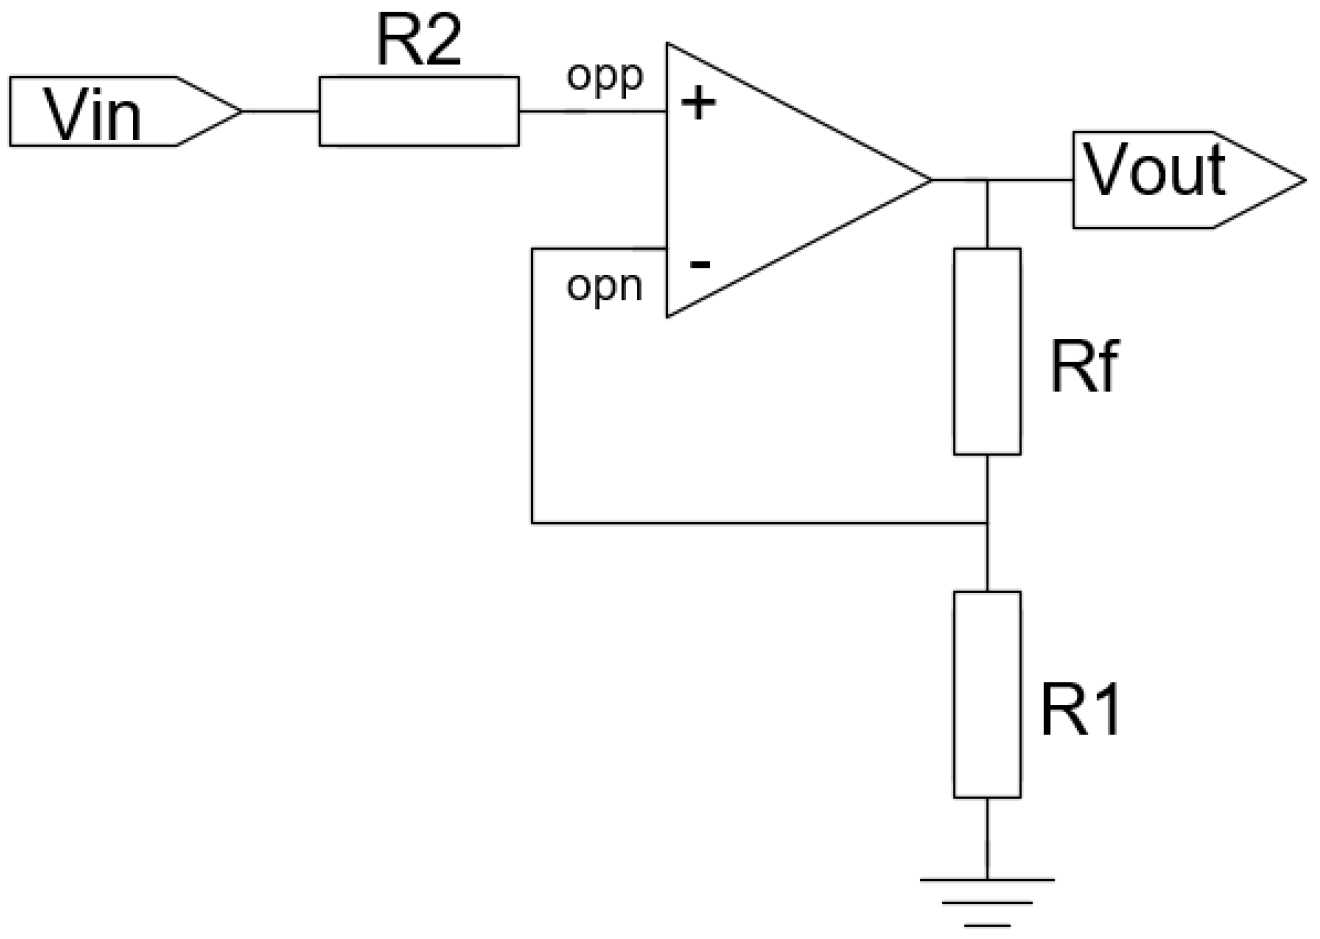
\includegraphics[width=\columnwidth]{images/kompensation_bias-strom_2.png}
		$$ R_2 = R_F || R_1 $$
	\end{center}
\end{minipage}
\hfill
\begin{minipage}[b]{0.3\columnwidth}
	\begin{center}
		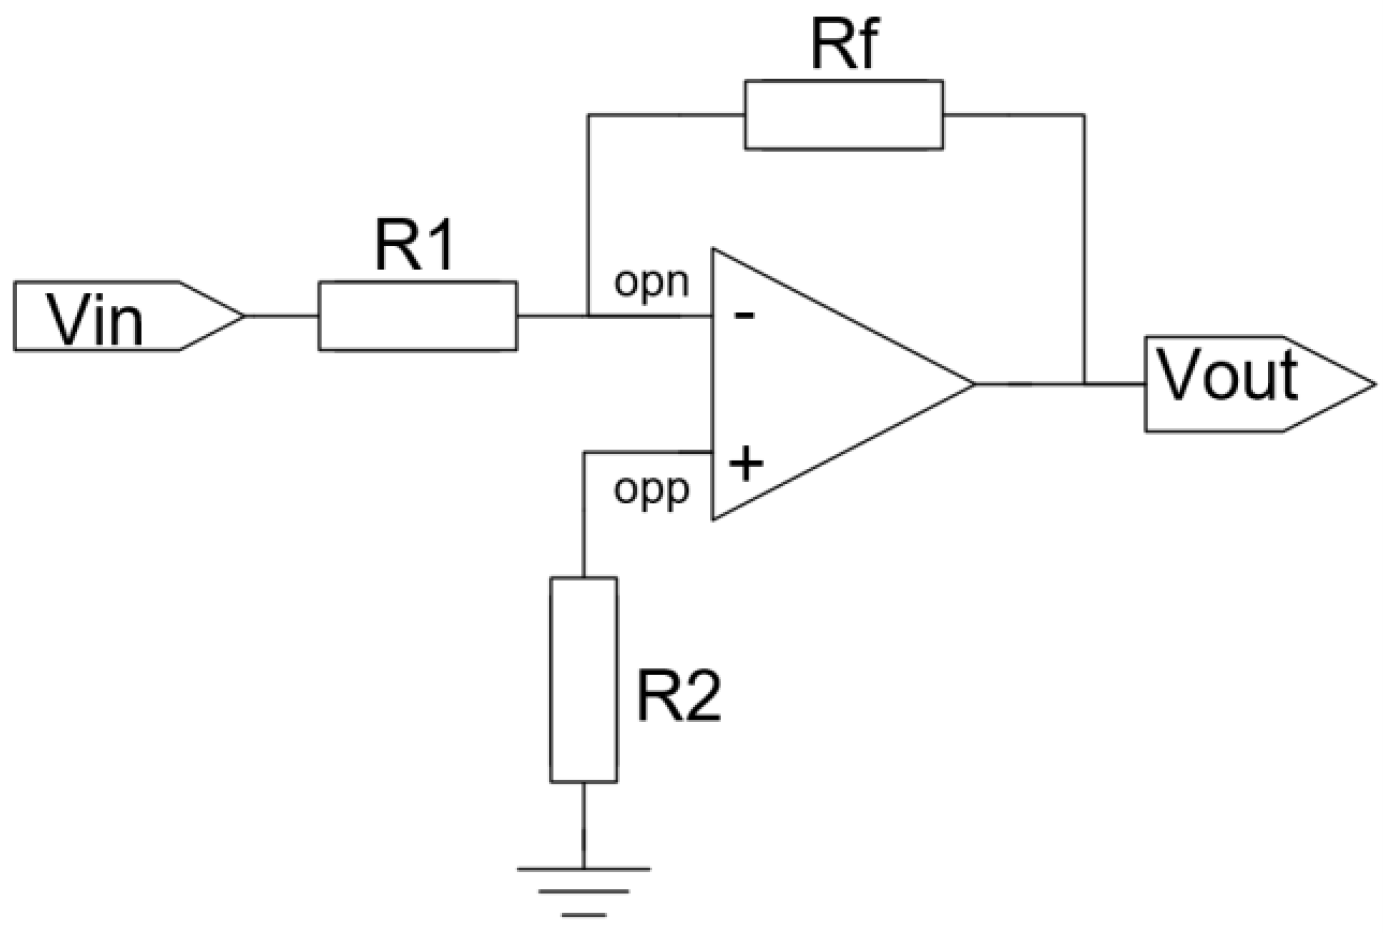
\includegraphics[width=\columnwidth]{images/kompensation_bias-strom_3.png}
		$$ R_2 = R_F || R_1 $$
	\end{center}
\end{minipage}


\subsubsection{Eingangsstromfehler - Offset-Strom $\bm{I_{\rm OS}}$}

Der Offset-Strom entsteht aufgrund von \textbf{Herstellungstoleranzen} und ist \textbf{nicht kompensierbar}
$$ \text{Offset-Strom:} \quad I_{\rm OS} = I_P - I_N $$

Wenn $I_B$ mittels $R_2$ kompensiert ist: \quad $\boxed{ |V_{\rm outE}| = R_F \cdot |I_{\rm OS}| } $

\textbf{\textrightarrow\ Je kleiner $\bm{R_F}$, desto kleiner die Fehlerspannung!}

\vspace{0.1cm}

\textbf{Gesamtfehler am Ausgang (worst case):} \quad $V_{\rm out,err} = \dfrac{|V_{\rm os}|}{\beta} + R_F \cdot |I_{\rm OS}|$


\subsection{Dynamisches Verhalten von OpAmps}

\subsubsection{Verstärkungs-Bandbreite-Produkt (GB(W)P)}

\begin{minipage}[c]{0.45\columnwidth}
	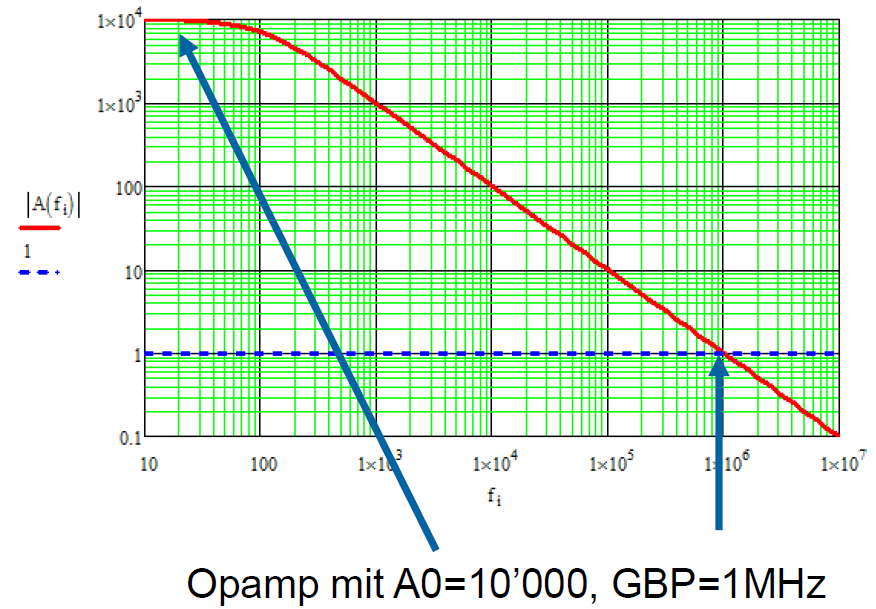
\includegraphics[width=\columnwidth]{images/verstaerkungs-bandbreite-produkt.png}
\end{minipage}
\hfill
\begin{minipage}[c]{0.52\columnwidth}
	$A_{\rm ol}$ sinkt mit der Frequenz (Tiefpass 1. Ordnung) \\
	\textrightarrow\ im Datenblatt GBWP statt $A_{\rm ol}$
	$$ A_{\rm ol}(f) \approx \frac{A_0}{1 + j \frac{f}{f_p}} \qquad \mathrm{GBWP} = A_0 \cdot f_p $$
	$$ \boxed{ A_{\rm cl} \cdot f_{3 \deci \bel} = \mathrm{GBWP} = \const } $$
\end{minipage}

\vspace{0.1cm}

Genau gilt mit der Noise Gain: \quad $\boxed{ f_{3 \deci \bel} = \beta \cdot \mathrm{GBWP} = \dfrac{\mathrm{GBWP}}{1 + R_2/R_1} }$ \\
Nicht-invertierend: $f_{3 \deci \bel} = \frac{\mathrm{GBWP}}{A}$ \qquad Invertierend: $f_{3 \deci \bel} = \frac{\mathrm{GBWP}}{1 + |A|}$ \\
Bsp.: GBWP $= 1 \, \mathrm{MHz}$, nicht-inv. mit $A = 10$ \textrightarrow\ $f_{3 \deci \bel} = 100 \, \mathrm{kHz}$


\subsubsection{Common Mode Rejection Ratio (CMRR)}

Unterdrückung von Gleichtaktsignalen (gleiche Spannung an beiden Eingängen)

\begin{minipage}[c]{0.48\columnwidth}
	$$ \boxed{ V_{\rm CM} = \frac{V_{\rm opp} + V_{\rm opn}}{2} } $$
	$$ \boxed{ \mathrm{CMRR} = \frac{\diff V_{\rm CM}}{\diff V_{\rm os}} } $$
\end{minipage}
\hfill
\begin{minipage}[c]{0.48\columnwidth}
	$$ \mathrm{CMRR} = \frac{A_D}{A_{\rm CM}} $$
	$$ \mathrm{CMRR_{dB}} = 20 \log (\mathrm{CMRR}) $$
\end{minipage}


\subsubsection{Power Supply Rejection Ratio (PSRR)}

Unterdrückung von Störungen auf der Versorgungsspannung
$$ \boxed{ \mathrm{PSRR} = \frac{\diff V_{\rm supply}}{\diff V_{\rm os}} } \qquad \mathrm{PSRR_{dB}} = 20 \log (\mathrm{PSRR}) $$


\subsection{Anstiegszeit (Slew-Rate)}

\begin{minipage}[c]{0.48\columnwidth}
	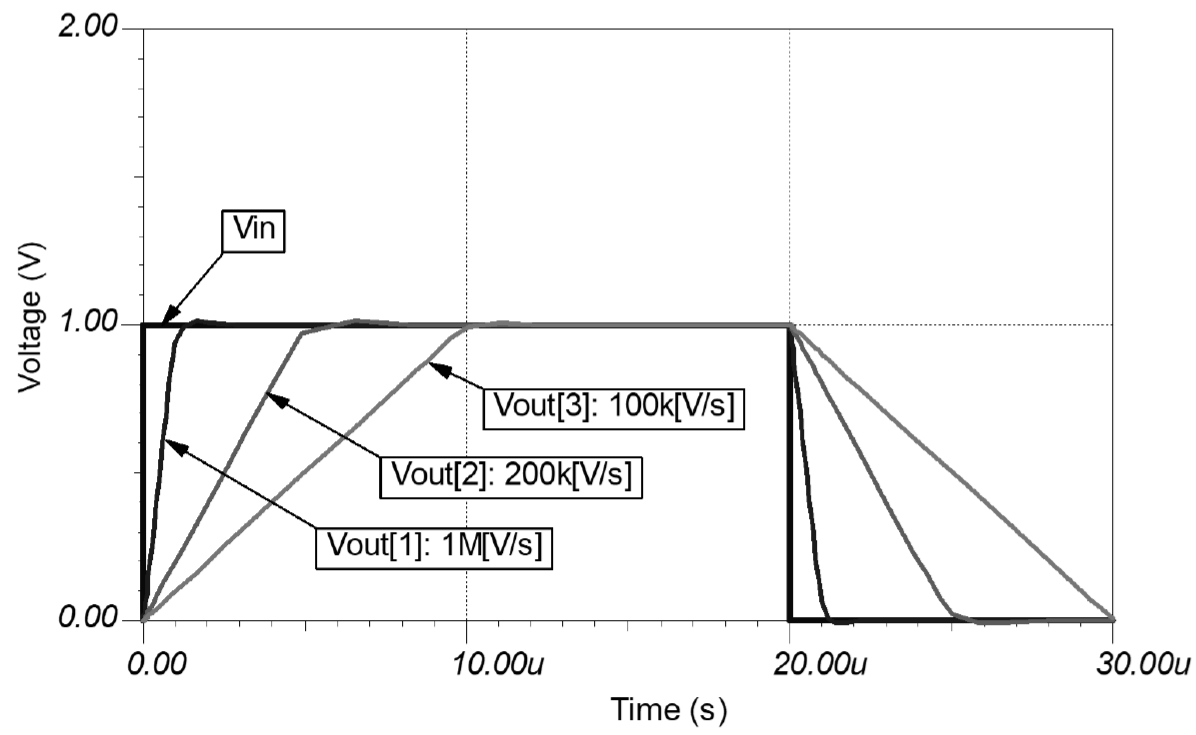
\includegraphics[width=\columnwidth]{images/slew_rate.png}
\end{minipage}
\hfill
\begin{minipage}[c]{0.48\columnwidth}
	\raggedright
	Maximal mögliche Änderungsgeschwindigkeit der Ausgangsspannung des OpAmps

	$$ \boxed{ \mathrm{SR} = \Bigl| \frac{\diff V_{\rm out}}{\diff t} \Bigr|_{\rm max} } $$
\end{minipage}

Wenn der Ausgang schneller ändern soll als die Slew-Rate 'erlaubt', so wird das Ausgangssignal \textbf{begrenzt bzw. verformt} \\
\textrightarrow\ Signal verformt / Amplitude reduziert \textrightarrow\ Dreieck statt Sinus

\textbf{Max. Frequenz für unverzerrten Sinus} (Amplitude $\hat{V}$): \quad
$\dfrac{\diff V}{\diff t}\Big|_{\rm max} = 2 \pi f \hat{V}$ \quad \textrightarrow\ \quad
$\boxed{ f_{\rm max} = \dfrac{\mathrm{SR}}{2 \pi \hat{V}} }$
